\documentclass[review]{elsarticle}
% \usepackage[utf8]{inputenc}
% \usepackage{subcaption}
% \usepackage{amsmath}
% \usepackage{listings}
% \usepackage{courier}
% \usepackage{tikz}
% \usepackage{graphicx}
% \usepackage{picins}
% \usepackage{epstopdf}
% 
% 
% \usepackage{lipsum}                        % testo fittizio
% 
% \usepackage[nomarkers]{endfloat}
% 
% \newcommand{\listoflstlistings}{\lstlistoflistings}
% \DeclareDelayedFloat{lstlisting}[flol]{\textbf{List of Listings}}
% 
% \lstset{tabsize=2,language=C++,basicstyle=\footnotesize\tt,keywordstyle=\color{blue}\bfseries}

\journal{Powder Technology}

%%%%%%%%%%%%%%%%%%%%%%%%%%%%%%%%%%%%%%%%%%%%%%%%%%%%%%%%%%%%%%%%%%%%%%%%%%%%%%%%%%%%%%%%%%%%%%%%%%%%%%%%%%%%%%%%%%%%%%%%%%
\begin{document}

%%%%%%%%%%%%%%%%%%%%%%%%%%%%%%%%%%%%%%%%%%%%%%%%%%%%%%%%%%%%%%%%%%%%%%%%%%%%%%%%%%%%%%%%%%%%%%%%%%%%%%%%%%%%%%%%%%%%%%%%%%
\begin{frontmatter}

\title{Identification of DEM Simulation Parameters by Artificial Neural Networks
and Bulk Experiments}

\author[jku]{L.~Benvenuti\corref{cor1}}
\ead{Tel. +43 73224686483}
\ead{luca.benvenuti@jku.at}

\author[dcs]{C.~Kloss}
\ead{christoph.kloss@dcs-computing.com}

\author[jku]{S.~Pirker}
\ead{stefan.pirker@jku.at}

\cortext[cor1]{Corresponding author}

\address[jku]{Johannes Kepler University Linz, Department on Particulate Flow
Modelling, Altenbergerstrasse 69, 4040, Linz, Austria}

\address[dcs]{DCS Computing GmbH, Altenbergerstr. 66a - Science Park, 4040 Linz,
Austria}

%%%%%%%%%%%%%%%%%%%%%%%%%%%%%%%%%%%%%%%%%%%%%%%%%%%%%%%%%%%%%%%%%%%%%%%%%%%%%%%%%%%%%%%%%%%%%%%%%%%%%%%%%%%%%%%%%%%%%%%%%%
\begin{abstract}
In Discrete Element Method ($DEM$) simulations, particle-particle contact laws
determine the macroscopic simulation results. Particle based contact laws, in
turn, commonly rely on semi-empirical parameters, which can be hardly obtained
by direct microscopic measurements.
In this study we present a methodology for the identification of
$DEM$ simulation parameters by linking the macroscopic experimental results to the
microscopic numerical parameters by artificial neural networks.
In a first step, a series
of $DEM$ simulations with varying simulation parameters are used to train a feed
forward artificial neural network by backward propagation reinforcement. In a
second step, this artificial neural network is utilized to predict the
macroscopic ensemble behaviour in dependence of additional sets of particle
based simulation parameters.
As a result, a comprehensive database is obtained,
which links particle based simulation parameters to a specific macroscopic
bulk behaviour of the ensemble.
The trained artificial neural network is able to predict the behaviour of
additional sets of input parameters accurately and highly efficient.
Furthermore, this methodology can be applied to
identify $DEM$ material parameters in a generic way.
For each set of calibration experiments, the training of the neural network has
to be performed just once. 
After the training, the neural network provides a generic link between the macroscopic 
experimental results and the microscopic $DEM$ simulation parameters.
By the help of these experiments, the $DEM$ simulation parameters of a specific
non-cohesive granular material can be identified.

\end{abstract}

\begin{keyword}
Discrete Element Method ($DEM$) Simulations \sep Parameter Identification \sep Artificial Neural Networks
\end{keyword}
\end{frontmatter}
%%%%%%%%%%%%%%%%%%%%%%%%%%%%%%%%%%%%%%%%%%%%%%%%%%%%%%%%%%%%%%%%%%%%%%%%%%%%%%%%%%%%%%%%%%%%%%%%%%%%%%%%%%%%%%%%%%%%%%%%%%

%************************************************
\section{Highlights}
\label{sec:highlights}
%************************************************
\begin{itemize}
  \item{We trained an Artificial Neural Network by DEM simulations with varying
  parameters}
  \item{The Artificial Neural Network then predicts granular bulk behaviour}
  \item{By comparison with bulk experiments DEM simulation parameters are
  identified}
  \item{This DEM parameter identification can be applied to different bulk
  behaviours}
  \item{This DEM parameter identification can be applied to different granular
  materials}
\end{itemize}
%************************************************

%% !TEX encoding = UTF-8
% !TEX TS-program = pdflatex
% !TEX root = ../elsarticle-template-num.tex
% !TEX spellcheck = en-EN

%************************************************
\section{Introduction}
\label{sec:introduction}
%************************************************

Particles in various forms - ranging from raw materials to food grains and pharmaceutical powders - play a major role in a variety of industries, including process industry and metallurgy. In his book, \citet{RefWorks:117} stated that "between 1 and 10\% of all the energy is used in comminution, i.e. the processes of crushing, grinding, milling, micronising". 
However, a univocal method to characterize these particles has so far not been established.
From the experimental point of view, the main issues are the difficult setups and the general reliability and reproducibility of the tests. 
From the numerical point of view, no general procedure is available, and the existence of a mathematically unique solution describing macro/micro particle contact has yet to be proved.
Moreover, in a recent study, \citet{RefWorks:56} implied "that the dynamic properties of a powder cannot be applied to universally predict the static properties of a powder, and, likewise, the static properties cannot be used to predict dynamic properties".\\
Discrete Element Method (DEM) simulations are widely used to understand particle behavior.
\citet{RefWorks:135} defined the $DEM$ as "a special class of numerical schemes for simulating the behavior of discrete, interacting bodies".
The force that particle i exerts on particle j is defined as:
\begin{equation}
m \ddot{x}_{ij} + c \dot{x}_{ij} + k x_{ij} =  F_{ij} .
\label{equ:newtonlaw}
\end{equation}

Further details on the method can be found in \citet{RefWorks:133}.
$LIGGGHTS$ (LAMMPS improved for general granular and granular heat transfer simulations) is one of the most powerful open source $DEM$ simulation software packages available. 
The models it can analyze are described in detail in the literature, see \citet{RefWorks:136}.\label{par:overviewdemliggghts}
In combination with shear cell tester simulation developed by \citet{RefWorks:139}, $LIGGGHTS$ has correctly defined the coefficient of sliding friction for coarse round particles - 
a critical parameter describing inter-particle friction in medium to dense granular flows simulations.\\
Since the bulk solid is represented by perfect spheres, the only parameter the software uses to describe its shape is the radius of the particle ($R$).
However, since the shape is one of the most relevant aspects defining particle behavior, we consider the coefficient of rolling friction ($\mu_r$) as an additional $DEM$ shape parameter. 
It is proportional to the torque counteracting the rotation of the particle and defined as (Eq. \ref{equ:mur}):
\begin{equation}
 \mu_r =  \tan(\iota) .
\label{equ:mur}
\end{equation}

The last $DEM-micro$ parameter investigated is the $coefficient-of-restitution$ ($COR$), given its centrality in the whole model.
$DEM$ simulations have recently been used to reduce the bias of the experiments, and more precise devices such as the Schulze ring shear cell tester (SRSCT)(see \citet{RefWorks:104}) have been built.
A dedicated workflow that combines experiments and simulations must now be devised following the Design of Experiments method, as illustrated by \citet{RefWorks:116}.\\
The main goal of this new procedure should be the characterization of non-spherical particles, especially the $DEM$ coefficients of friction and restitution, following standardizable steps.
With this objective in mind, we profited from the shear cell experimental and numerical setup in combination with $LIGGGHTS$ simulation to improve the accuracy and the range of applicability of particle characterization.
Nevertheless, $DEM$ simulations require tens of thousand of particles to achieve the necessary reliability for a straight-forward trial-and-error calibration procedure.
The calibration compels to identify the $DEM-micro$ combination of parameters that numerically grants the same $bulk-macro$ behavior experimentally registered, measured as $steady-state-flow/pre-shear ~ coefficient-of-internal-friction $ $ (\mu_{ie-ps})$, $incipient-flow/shear ~ coefficient-of-internal-friction $ $ (\mu_{ie-s})$ and $bulk ~ density ~ (\rho_b)$.
Furthermore, we used Hertz' Law for the particle-particle and particle-wall interactions.
Its complexity increased the computational effort to fathom the micro-macro transition relationship. 
Thus, the time necessary to perform all the possible $DEM-micro$ parameters combinations became boundless.
In order to overcome this doomed situation we decided to operate artificial neural networks, as suggested by \citet{RefWorks:161}.
A limited number of combinations have been simulated, designed to maxime the representativity.
Following the indications of \citet{RefWorks:150}, \textit{feed forward Multilayer Perceptron Neural Networks (MLPNN)} have been handled.
Their trustworthiness, together with a backpropagation reinforcement learning training algorithm(scaled conjugate gradient), has been widely demonstrated in the literature, see \citet{RefWorks:158}.
The DEM parameters of the simulations have been used as inputs of the Neural Networks ($NN$), while the bulk values and behavior as targets for them.
Furthermore, the best practice suggested by \citet{RefWorks:150} demands to establish the most appropriate number of neurons inside the hidden layer of each $NN$.
As in literature, this goal has been achieved by first excluding 15\% of the simulations from the training processes.
We then fed the $NN$ with the same $DEM-micro$ parameters of these simulations.
Subsequently, we controlled the square regression error between the $bulk-macro$ behavior in these simulations and in the output of the $NN$.
Finally, we selected for each $bulk-macro$ behavior property ($\mu_{ie-ps}$, $\mu_{ie-s}$ and $\rho_b$) the $NN$ with the number of neurons that provided the maximum $R^2$.
Later, each of these three trained $NN$ received as insertion $1M$ different combinations $DEM-micro$ parameters.
We then compared their outputs against the values provided by the shear cell experiments (within a 5\% error), gaining the $DEM-micro$ coefficients range.
\citet{RefWorks:160} prescribes an ulterior validation step.
To accomplish his demand, we realized a $static-angle-of-repose$ ($SAOR$) experiment and $SAOR$ simulation.
Furthermore, we performed the $SAOR$ simulation, again with the same limited number of combinations.
These allowed to determine two $bulk-macro$ behavior properties, the $angle-of-repose$ ($AOR$) and the $bulk ~ density ~ (\rho_b)$.
Likewise, we then trained $NN$ and optimized the number of their neurons.
Later, each of these two trained $NN$ received as insertion the $DEM-micro$ coefficients range previously determined.
We then compared their outputs against the values provided by the $SAOR$ experiment (again within a 5\% error), gaining a narrower $DEM-micro$ coefficients range.
Since this study was supported by the metallurgical industry, the materials examined were: silibeads (2 mm), coke, iron ore, limestone (all 0-3.15 mm).
For the same reason, cohesive materials have been excluded from this study.\\ \label{par:materials}
trotaculo bis


%\section{Modelling Pre-requisites}
\label{sec:modellingprerequisites}
%************************************************
%\section{Method}
%\label{sec:method}
%************************************************

%%%\lipsum[1]
%%\begin{equation}
\label{eq:emc}
e = mc^2
\end{equation}


\subsection{Macroscopic Experiments}
\label{subsec:Macroscopicexperiments}

The first step of the procedure was using a SRSCT (see \cite{RefWorks:142}) to characterize particle flow properties, 
especially the complete yield locus.
With the procedure described in \ref{subsec:srsctexperiment} we
obtained for each of the twelve load conditions three values representative of the bulk behaviour: bulk density ($\rho_b$),
coefficient of internal friction in the pre-shear phase $ (\mu_{psh})$ and
coefficient of internal friction in the shear phase  $ (\mu_{sh})$.\\
Furthermore, in order to recreate the repose angle observed in a pile of the real material, 
we performed angle of repose ($AOR$) tests, as the $AOR$ was the fourth
behaviour value. The complete description can be found in
\ref{subsec:aorexperiment}.
Moreover, we sieved the materials samples to obtain the size distribution of the
particles. Six different sifters have been used.\\

\subsection{Discrete element method}
\label{subsec:dem}
The $DEM$ is based on a relatively elementary idea. 
For each particle i inside the domain it follows the trajectory and calculates the force that particle i exerts on particle j. 
The main forces involved are: gravity, contact forces due to collisions and further interactions such as electrostatic, 
Van der Waals, cohesive forces and fluid-solid interactions in multiphase flows. For the raw material used in this work 
Di Renzo and Di Maio \cite{RefWorks:145} suggested using the non-linear Hertzian model without cohesion for 
the particle-particle and particle-wall contacts. 
This granular model uses the following formula for the contact force between two granular particles (Eq. \ref{eq:forceij}):
\begin{equation}
 F_{ij} = 
\begin{cases}
F_{n,ij} + F_{t,ij} = \left( k_n \delta_{n,ij} + \gamma_n v_{n,ij} \right) + \left( k_t \delta_{t,ij} + \gamma_t v_{t,ij} \right) & \text{if } r < d ,\\
0    & \text{if } r > d ,\\
\end{cases}
 \label{eq:forceij}
\end{equation}

where the subscript n stands for normal and t for tangential. 
$k$ and $\gamma$ are respectively the elastic and damping coefficients, 
while $\delta$ and $v$ the displacement and the velocity, $r$ the distance
between two particles of radii $R_i$ and $R_j$ and $d = R_i + R_j $ is the
contact distance.
Both the normal and the tangential
force comprise two terms, a spring force and a damping force. 
The shear force is a "history" effect that accounts for the tangential displacement 
("tangential overlap") between the particles for the duration of contact. 
The tangential force component is truncated to fulfil 
\begin{equation}
F_{t,ij} \leq \mu_s F_{n,ij},
 \label{eq:force_t}
\end{equation}

where $\mu_s$ is the coefficient of sliding friction, one of the particle based
DEM parameter we investigated. 
An ulterior parameter was the coefficient of rolling friction ($\mu_r$). 
For coarse not round particles is a critical parameter and describes inter-particle 
friction in medium to dense granular flows simulations. It is proportional to the 
torque counteracting the rotation of the particle. The $\mu_r$ parameter enters the 
equations according to the elasto-rolling resistance model presented by Wensrich and 
Katterfeld \cite{RefWorks:87} and Ai et al. \cite{RefWorks:131}, 
based on the work of Jiang et al. \cite{RefWorks:143}. 
The model is called $EPSD2$ in $LIGGGHTS$. This is appropriate for the one way
rolling cases as well as the cycling rolling ones.
The maximum magnitude of rolling resistance torque is (Eq. \ref{eq:trmax}):
\begin{equation}
T_{r~max} = \mu_r R_r |\tilde{F_n}| ~,
 \label{eq:trmax}
\end{equation}

where $R_r$ is the equivalent radius and $F_n$ the normal force.
The DEM parameters for the Young's modulus ($E$) and the coefficient of Poisson ($\nu$) 
have been taken from the literature, see \cite{RefWorks:175} and \cite{RefWorks:176}, 
although we reduced the former to increase the time step, following the indications of Ai et al. \cite{RefWorks:131}. 
The particles radii have been approximated from the experimental measurements. 
The last two particle based $DEM$ parameter we investigated were the particle density 
($\rho_p$) and the coefficient of restitution ($COR$), as defined by Ai. et al. \cite{RefWorks:131}. 
There and in the work Wensrich and Katterfeld \cite{RefWorks:87} further details on the method can be found.
The complete description of the shear cell simulations can be found in \ref{subsec:srsctsimulation}, 
while the AOR simulation is presented in appendix \ref{subsec:aorsimulation}.\\

\subsection{Artificial Neural Networks}
\label{subsec:ann}

An Artificial Neural Network ($NN$) is a powerful modellization technique, 
based on non-linear functions (Haykin \cite{RefWorks:158}). 
In this paper, we first use the $NN$ to fit the $DEM$ numerical simulation data, 
and then to process vast amount of parameters combinations. 
The original idea is directly borrowed from human brain design, with neurons and synapses. 
They map combinations of input data into convenient outputs (fitting). 
There is a variety of types of $NN$, remarkably the Feedforward ($FF$) 
and the Radial basis function ($RBF$). For $FF-NN$, considerable amount 
of traning algorithms are available. The most common are based on backpropagation: 
e.g. Levenberg-Marquardt, Bayesian regulation and scaled conjugate gradient. 
To recognize not linearly separable data the standard linear perceptron $NN$ 
has been modified into \textit{FF Multilayer Perceptron Neural Networks (MLPNN)}. 
Here, each processing units or node (neuron) possesses a nonlinear activation function. 
Together, they are interconnected into layers, also linked together. 
The trustworthiness of the $MLPNN$, with a backpropagation reinforcement learning 
training algorithm (scaled conjugate gradient), has been widely demonstrated in the 
literature, see Haykin \cite{RefWorks:158}. Several scientists 
\cite{RefWorks:161, RefWorks:166, RefWorks:167, RefWorks:168, RefWorks:169, RefWorks:170} 
have operated $NN$ to model materials mechanical properties. 
In fact, $MLPNN$ are built with three different layers. 
\begin{figure}[!htb] 
\centering 
\includegraphics[width=.96\textwidth]{images/original/18NNscheme} 
\caption{NN scheme}
\label{fig:18NNscheme} 
\end{figure}


% \begin{figure}[htp]
%     \centering
%     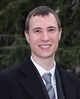
\includegraphics[width=.2\textwidth]{images/vitae/lbenvenuti}
%     \caption{OpenMP, MPI, MPI/OpenMP Hybrid runs of Box in a box testcase on 32
%     cores. The OpenMP-only run suffers from limited memory bandwidth in
%     memory-bound algorithms inside of the Modify section of the code. MPI-only has
%     low averaged runtimes for each section, but a very large Other timing, which
%     hints for a large amount of load-imbalance. Hybrid timings are a bit worse
%     on average, but because of better balancing, processes have lower wait times
%     inside of Other timing.}
% 	\label{fig:boxInBoxComparison}

The input layer has a number of neurons equal to the number of different inputs
of the network, see Fig. \ref{fig:18NNscheme}.
Following the best practice suggested by Vaferi et al. \cite{RefWorks:150} $MLPNN$ have been handled.
Similarly, the best practice also demands to establish the most appropriate number of neurons inside the 
hidden layer of each $NN$. This check has been handled through mean square maximization ($R^2$). 
For each investigated output we chose the number of neurons with the greater
$R^2$.\\
Further, we should question the quality of the NN data, accordingly to the 
Oberkampf et al. \cite{RefWorks:160} method. Haykin \cite{RefWorks:158} 
suggests questioning both the NN training process and the following data generation from given inputs. 
The former is usually challenged when dealing with experimental training data, and frequently 
managed by noise-corrupted patterns calibration. Nevertheless, our training pool is numerical. 
The particles in each of our simulations are created through a random algorithm, and the training pool is extensive. 
For massive training data the effect of noise-corrupted patterns is negligible, see Haykin \cite{RefWorks:158}. 
Instead the latter was a challenging aspect of our work. Once trained, as input for the $NN$ we imposed 
combinations of $DEM$ parameters. 
We tried different methods to generate these combinations. 
Our first attempt was assigning to the investigated variables parameters in even increments 
from the minimum to the maximum values. 
E.g. the $COR$ ranges from 0.5 to 0.9, the first value would be 0.5, the second 0.508163 and so on. 
To increase the generalization, we decided to follow a different approach. 
Random values generators created values in the defined ranges and in the requested 
number for each of the investigated parameter. Then, they were combined and imposed as input.\\

%\section{Methodology of DEM Parameter Identification}
\label{sec:methodology}

We now illustrate the methodology used, also shown in Fig.
\ref{fig:19methodology}.
%\begin{figure}[!htb] 
\centering 
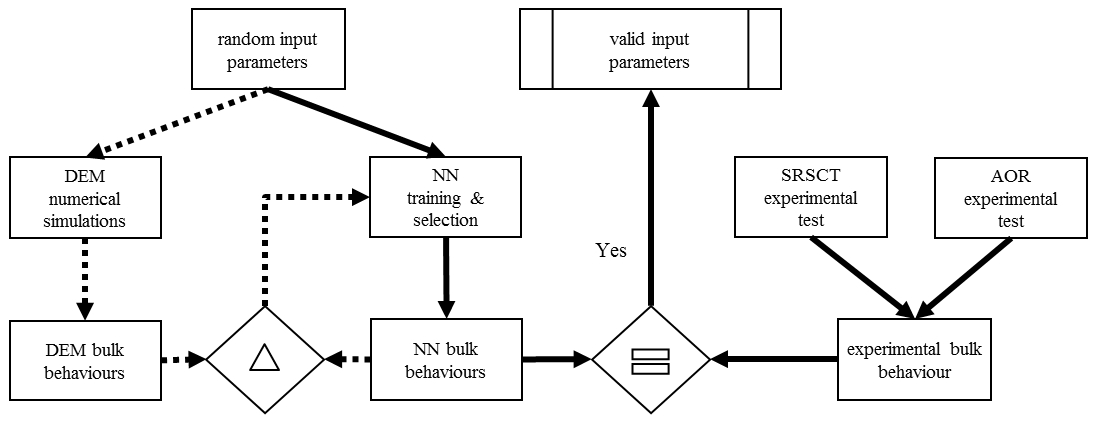
\includegraphics[width=.96\textwidth]{19methodology} 
\caption[Methodology]{Methodology. 
In the training phase (dashed lines) from the initial random input parameters
$DEM$ simulations are performed. The behaviours provided are used to train the
Neural Networks ($NN$), in a loop that continues until the difference is within
the limit ($\Delta$).
Then in the parameters' identification phase (straight
lines) we identify the valid input parameters by comparing (\textbf{=}) $NN$ and
experimental behaviours.
Further explanations in the text.
}
\label{fig:19methodology} 
\end{figure}


% \begin{figure}[htp]
%     \centering
%     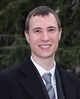
\includegraphics[width=.2\textwidth]{images/vitae/lbenvenuti}
%     \caption{OpenMP, MPI, MPI/OpenMP Hybrid runs of Box in a box testcase on 32
%     cores. The OpenMP-only run suffers from limited memory bandwidth in
%     memory-bound algorithms inside of the Modify section of the code. MPI-only has
%     low averaged runtimes for each section, but a very large Other timing, which
%     hints for a large amount of load-imbalance. Hybrid timings are a bit worse
%     on average, but because of better balancing, processes have lower wait times
%     inside of Other timing.}
% 	\label{fig:boxInBoxComparison}



% After the $DEM$ simulations the Neural
% Network ($NN$) are trained and selected. We then compare experimental and
% numerical results to identify the valid parameters.
The experimental characterization has been performed as described in
\ref{subsec:srsctexperiment} and \ref{subsec:aorexperiment}. We performed
three tests with the $SRSCT$ for the sinter fine bulk, for a total of twelve
load conditions. 
%An example for three of them can be seen in table
% \ref{tab:05sinterTableExperimental}.
% \begin{table}[h]
\centering
\begin{tabular}{cccccc}
\hline
$\sigma_n$ (Pa) & $\tau$ (Pa) & $\mu_{psh}$ (-) & $\tau_{\%}$ (\%) &
$\mu_{sh}$ (-) & $\rho_b$ (kg/m3) \\
\hline
    1068  & 1059  & 0.9916 & 80 & 1.2333 & 1718 \\
    2069  & 1818  & 0.8787 & 80 & 0.9994 & 1759 \\
    10070 & 8232  & 0.8175 & 80 & 1.1712 & 1802 \\

\hline
\end{tabular}
\caption[Experimental results]{Experimental results. Values for three
load conditions}
\label{tab:05sinterTableExperimental}
\end{table}
The first bulk behaviour representative value ($\rho_b$) was directly provided. 
If the test was performed correctly, see \ref{subsec:srsctexperiment}, we
observed a linear increase in the coefficient of internal friction.
%, see Fig. \ref{fig:20experimental}.
Later, the first plateau was reached. 
The second bulk behaviour representative value ($\mu_{psh}$) was calculated by averaging the coefficient in this plateau. 
Further, the normal load was modified, and then a second plateau was reached. The third value ($\mu_{sh}$) was 
determined by averaging the coefficient in this plateau. 
Next, we performed two $AOR$ tests. 
The average of the repose angles provided us the fourth bulk value, allowing us
to define the experimental bulk behaviour.
For simulations purposes, we also sieved the bulk to know the size distribution.
We could then focus on the simulations. 
As stated in the modelling section of this paper, we decided to fix one single
contact law for all the simulations performed.
Furthermore, we locked the size distribution, as provided by the sieving, the
elastic coefficients and the time step, see table
\ref{tab:09DEMFixedinputvalues}.
% \begin{table}[h]
\centering
\begin{tabular}{ccc}
\hline
    Young's & Poisson's & \acs{deltat}\\
   modulus & ratio & \\
    $[MPa]$ & $[-]$ & [s]\\
    \hline
    $10$    & $0.40$ & $10^{-6}$\\


\hline
\end{tabular}
\caption{DEM fixed input values}
\label{tab:09DEMFixedinputvalues}
\end{table}
% \begin{table}[h]
\centering
\begin{tabular}{ccccc}
\hline
    \acs{mus} & \acs{mur} & \acs{CoR} & \acs{rhop} & \acs{dCylDp} \\
    	$[-]$  & $[-]$   & $[-]$   & $[kg/m3]$ & $[-]$ \\
    \hline
    0.4 / 0.6 / 0.8 & 0.4 / 0.6 / 0.8 & 0.5 / 0.7 / 0.9 & 2500 / 3000 / 3500 & 20 / 36 / 38 / 40 \\

\hline
\end{tabular}
\caption[DEM variable input values]{DEM variable input values for training the
Neural Networks}
\label{tab:10DEMVariableinputvalues}
\end{table}
The last was between $1.29 \%$ and $1.53 \%$ of the Rayleigh time, that depends
to the particle density.
Other coefficients, $COR$, $\mu_s$, $\mu_r$,
$\rho_p$ and $dCylDp$, as indicated in table \ref{tab:10DEMVariableinputvalues},
were constant in each simulation, but their combination differed between
simulations.
%, see e.g. table \ref{tab:11DEMSimExampleinputvalues}.
% \begin{table}[h]
\centering
\begin{tabular}{lccccc}
\hline
 sim &  $\mu_s$ & $\mu_r$ & $COR$ & $\rho_p$ & $dCylDp$ \\
  \#  &	$[-]$  & $[-]$   & $[-]$   & $[kg/m3]$ & $[-]$ \\
          \hline
    1st & 0.40  & 0.40  & 0.50  & 2500  & 20 \\
    2nd & 0.60  & 0.40  & 0.50  & 2500  & 20 \\


\hline
\end{tabular}
\caption{DEM simulation examples input values}
\label{tab:11DEMSimExampleinputvalues}
\end{table}
Further, $dCylDp$ was used to evaluate the wall effect, but only $~10\%$ of the
all simulations had $dCylDp$ larger than $20$ (additional information can be found in \ref{subsec:srsctsimulation}). 
The normal stress $\sigma_n$ and its
percentage during the incipient flow condition $\tau_{\%}$
varied to replicate the twelve shear cell load conditions. 
In total, we realized $546$ shear cell and $81$ angle of repose simulations.
A Matlab script allowed us to extract from the simulations output the numerical
bulk representative values ($\mu_{psh}$, $\mu_{sh}$, $\rho_b$ and $AOR$) for each $simulation-DEM$ parameter combination. 
So, we could use the $DEM$ parameter combinations and their corresponding bulk values to train the $NN$. 
Notably, we excluded 15\% of the simulations ($test ~ simulations$), randomly
picked, from the training processes.
First, we started with all the $DEM$ parameter combinations and their corresponding numerical $\mu_{psh}$ to create 36 $NN$. 
They differed because they included from five to forty neurons in the hidden
layer.
Later, we controlled the square regression error between the $bulk-macro$ behaviours in the output of 
the $NN$ and the 15\% $test ~ simulations$, granted uncorrelated. 
So, we could select for $\mu_{psh}$ the $NN$ with the maximum $R^2$, and we noted its number of neurons. 
We repeated the same steps from the $NN$ creations for $\mu_{sh}$, $\rho_b$ and $AOR$, 
obtaining one trained $NN$ for each bulk representative value. \\
% \begin{table}[h]
\centering
\begin{tabular}{lcccc}
\hline
 &  \ac{mus} & \ac{mur} & \ac{CoR} & \ac{rhop}  \\
  &	$[-]$  & $[-]$   & $[-]$   & $[kg/m3]$ \\
          \hline
    range & $[0.1 \ldots 1.0]$ & $[0.1 \ldots 1.0]$ & $[0.5 \ldots 0.9]$ &
    $[2000 \ldots 3500]$     \\
    \# rnd & 100   & 100   & 25    & 25    \\

\hline
\end{tabular}
\caption[DEM random input values]{DEM random input values. Within each range \#
random values are chosen.}
\label{tab:12DEMRandominputvalues}
\end{table}
Notably, $\mu_{psh}$, $\mu_{sh}$ and $\rho_b$ belonged to the shear cell
simulations, so their $NN$ were handled together. We then created random values
in the range and number defined in table \ref{tab:12DEMRandominputvalues}.
The total number of combinations of these random values was $6250000$. These
combinations were then processed by the selected $NN$, granting for each three bulk representative parameters for the shear cell and one for the $AOR$. Later, we confronted the $NN$ and experimental bulk behaviours for the twelve shear cell load conditions. 
If in a $DEM-parameter$ combination all the three bulk representative parameters differed less 
than 5\% from the corresponding experiments, see Eq. \ref{eq:check2}:
\begin{equation}
 \begin{cases}
\text{if } & \lvert{1-\frac{\mu_{psh,num}}{\mu_{psh,exp}}}\rvert < 5\%  ,\\
\text{and if } & \lvert{1-\frac{\mu_{sh,num}}{\mu_{sh,exp}}}\rvert < 5\% , \\ 
\text{and if } & \lvert{1-\frac{\rho_{p,num}}{\rho_{p,exp}}}\rvert < 5\% ,\\ 
\end{cases}
 \label{eq:check2}
\end{equation}
then the combination was tabbed. The latter combinations were handled by the $AOR$ $NN$, and then confronted with the experiment. 
Were branded as valid only those that differed less than $5\%$ also in this
comparison (Eq. \ref{eq:checkaor}):
\begin{equation}
\text{if} ~~~~~~ \lvert{1-\frac{AoR_{num}}{AoR_{exp}}}\rvert < 5\% .
\label{eq:checkaor}
\end{equation}
%************************************************
Further, to prove the system validity, we tested the tabbed combinations by modifying the experimental bulk
behaviour representative values of the shear cell. 
We artificially decreased or increased $\mu_{psh}$ and $\mu_{sh}$ by a product
coefficient ($P$), e.g. Eq. \ref{eq:pcoeff}:
\begin{equation}
\label{eq:pcoeff}
\mu_{psh, new} = \mu_{psh, old} \cdot P .
\end{equation}

\begin{figure}[!htb] 
\centering 
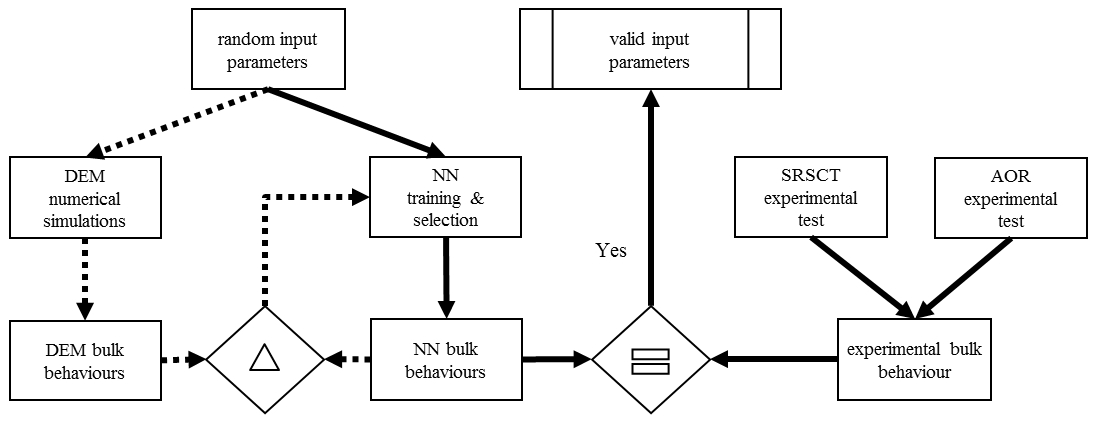
\includegraphics[width=.96\textwidth]{19methodology} 
\caption[Methodology]{Methodology. 
In the training phase (dashed lines) from the initial random input parameters
$DEM$ simulations are performed. The behaviours provided are used to train the
Neural Networks ($NN$), in a loop that continues until the difference is within
the limit ($\Delta$).
Then in the parameters' identification phase (straight
lines) we identify the valid input parameters by comparing (\textbf{=}) $NN$ and
experimental behaviours.
Further explanations in the text.
}
\label{fig:19methodology} 
\end{figure}


% \begin{figure}[htp]
%     \centering
%     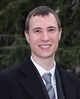
\includegraphics[width=.2\textwidth]{images/vitae/lbenvenuti}
%     \caption{OpenMP, MPI, MPI/OpenMP Hybrid runs of Box in a box testcase on 32
%     cores. The OpenMP-only run suffers from limited memory bandwidth in
%     memory-bound algorithms inside of the Modify section of the code. MPI-only has
%     low averaged runtimes for each section, but a very large Other timing, which
%     hints for a large amount of load-imbalance. Hybrid timings are a bit worse
%     on average, but because of better balancing, processes have lower wait times
%     inside of Other timing.}
% 	\label{fig:boxInBoxComparison}



% After the $DEM$ simulations the Neural
% Network ($NN$) are trained and selected. We then compare experimental and
% numerical results to identify the valid parameters.

\begin{table}[h]
\centering
\begin{tabular}{ccc}
\hline
    Young's & Poisson's & \acs{deltat}\\
   modulus & ratio & \\
    $[MPa]$ & $[-]$ & [s]\\
    \hline
    $10$    & $0.40$ & $10^{-6}$\\


\hline
\end{tabular}
\caption{DEM fixed input values}
\label{tab:09DEMFixedinputvalues}
\end{table}
\begin{table}[h]
\centering
\begin{tabular}{ccccc}
\hline
    \acs{mus} & \acs{mur} & \acs{CoR} & \acs{rhop} & \acs{dCylDp} \\
    	$[-]$  & $[-]$   & $[-]$   & $[kg/m3]$ & $[-]$ \\
    \hline
    0.4 / 0.6 / 0.8 & 0.4 / 0.6 / 0.8 & 0.5 / 0.7 / 0.9 & 2500 / 3000 / 3500 & 20 / 36 / 38 / 40 \\

\hline
\end{tabular}
\caption[DEM variable input values]{DEM variable input values for training the
Neural Networks}
\label{tab:10DEMVariableinputvalues}
\end{table}
%\begin{table}[h]
\centering
\begin{tabular}{lccccc}
\hline
 sim &  $\mu_s$ & $\mu_r$ & $COR$ & $\rho_p$ & $dCylDp$ \\
  \#  &	$[-]$  & $[-]$   & $[-]$   & $[kg/m3]$ & $[-]$ \\
          \hline
    1st & 0.40  & 0.40  & 0.50  & 2500  & 20 \\
    2nd & 0.60  & 0.40  & 0.50  & 2500  & 20 \\


\hline
\end{tabular}
\caption{DEM simulation examples input values}
\label{tab:11DEMSimExampleinputvalues}
\end{table}
\begin{table}[h]
\centering
\begin{tabular}{lcccc}
\hline
 &  \ac{mus} & \ac{mur} & \ac{CoR} & \ac{rhop}  \\
  &	$[-]$  & $[-]$   & $[-]$   & $[kg/m3]$ \\
          \hline
    range & $[0.1 \ldots 1.0]$ & $[0.1 \ldots 1.0]$ & $[0.5 \ldots 0.9]$ &
    $[2000 \ldots 3500]$     \\
    \# rnd & 100   & 100   & 25    & 25    \\

\hline
\end{tabular}
\caption[DEM random input values]{DEM random input values. Within each range \#
random values are chosen.}
\label{tab:12DEMRandominputvalues}
\end{table}
%\section{Results and discussion}
\label{sec:results}
%************************************************

\subsection{Experiments}
\label{subsec:experiments}

Initially, experimental values identifying the bulk behavior, $\mu_{psh}$, $\mu_{sh}$ and $\rho_{b}$, 
for sinter fine have been acquired through the $SRSCT$, e.g. in Table
\ref{tab:05sinterTableExperimental}
these values for three load conditions are presented.
In the $\mu_{psh}$ a descending path is evident. 
Instead, the $\mu_{sh}$ is oscillating.
The $\rho_b$ presents a clear average of $1760 [kg/m^3]$ with a $42 [kg/m^3]$
deviation.
The stress path for the second load condition of Table
\ref{tab:05sinterTableExperimental} is shown in Fig.
\ref{fig:20experimental}.
In the first 300 seconds the $\sigma_n$ was kept constant. After 250 seconds a
plateau was reached. 
The $\mu_{psh}$ was calculated as average of the $\mu_{ie}$ in this plateau.
Later, the $\sigma_n$ was reduced to $80 \%$ of its initial value.
After approximately 30 seconds, a second plateau started.
As average of $\mu_{ie}$ in this second plateau we obtained $\mu_{sh}$.
Later, two $AOR$ test have been performed, thus identifying an average angle of
$38.85 ^\circ$.
We also realized the sieving, obtaining the radius ($R$) mean and standard
deviation, already shown in Table \ref{tab:09DEMFixedinputvalues}.
\begin{figure}[htp] \centering
    \begin{subfigure}[b]{2cm}
        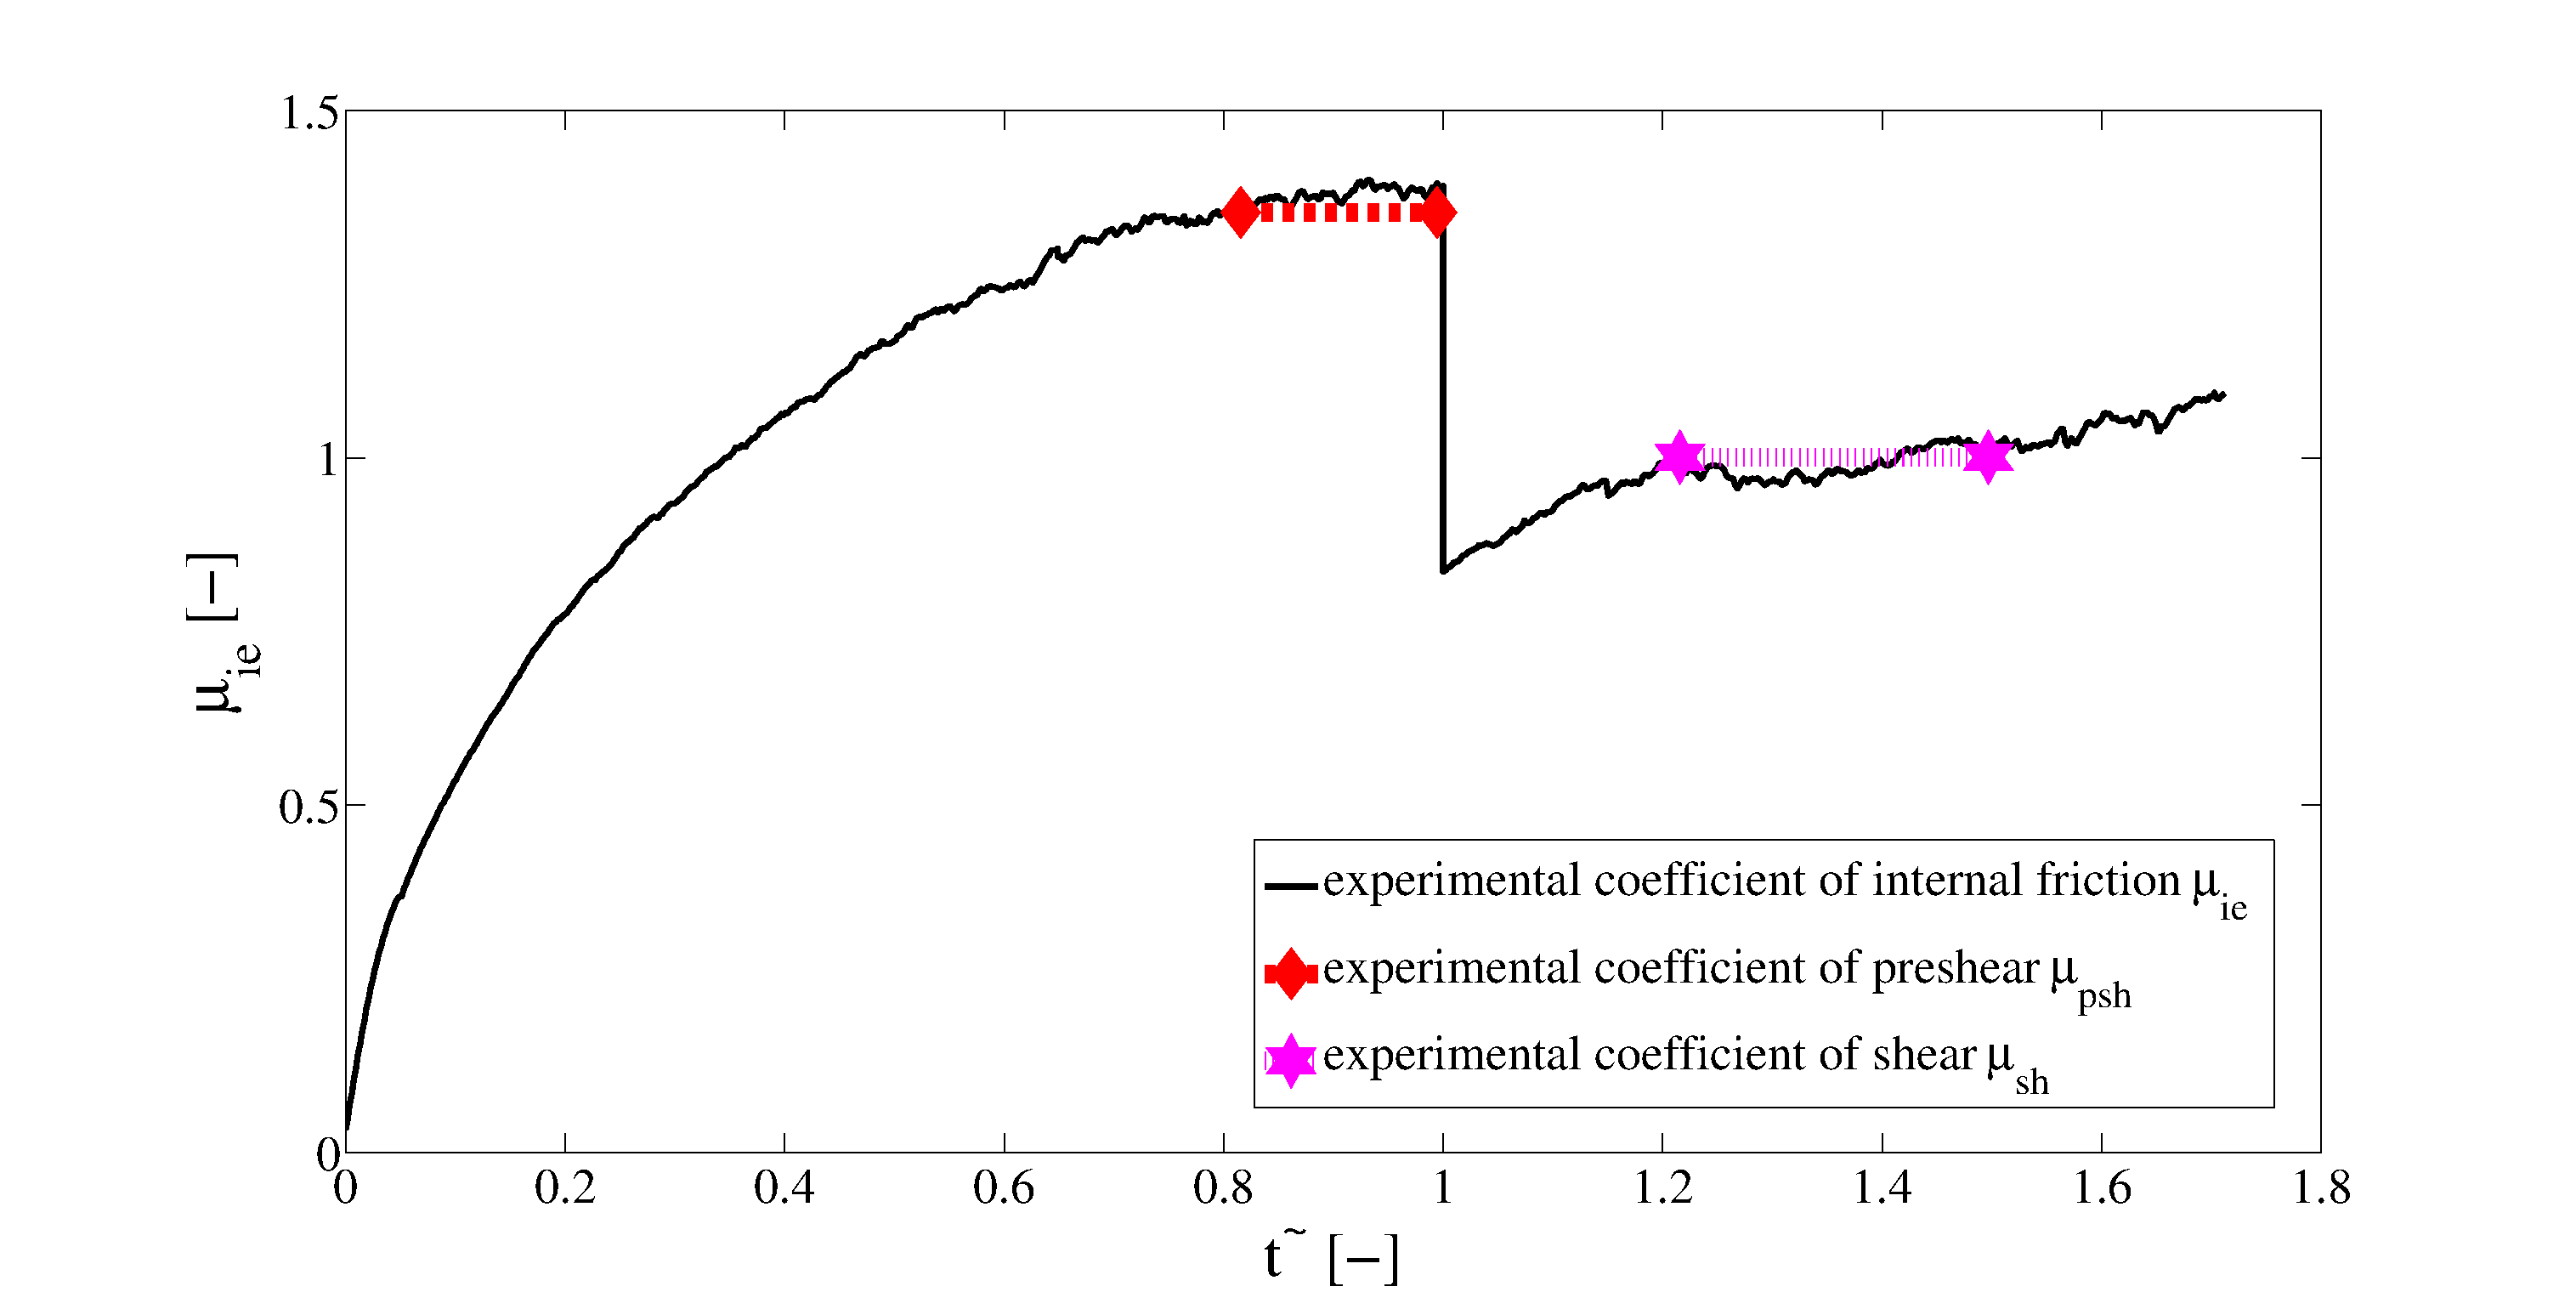
\includegraphics[width=\textwidth]{images/original/20experimental}
        \caption{Experimental shear cell tester stress path - $\sigma_n = 2000
        [Pa]$}
        \label{fig:20experimental} 
    \end{subfigure}\\
        \begin{subfigure}[b]{2cm}
        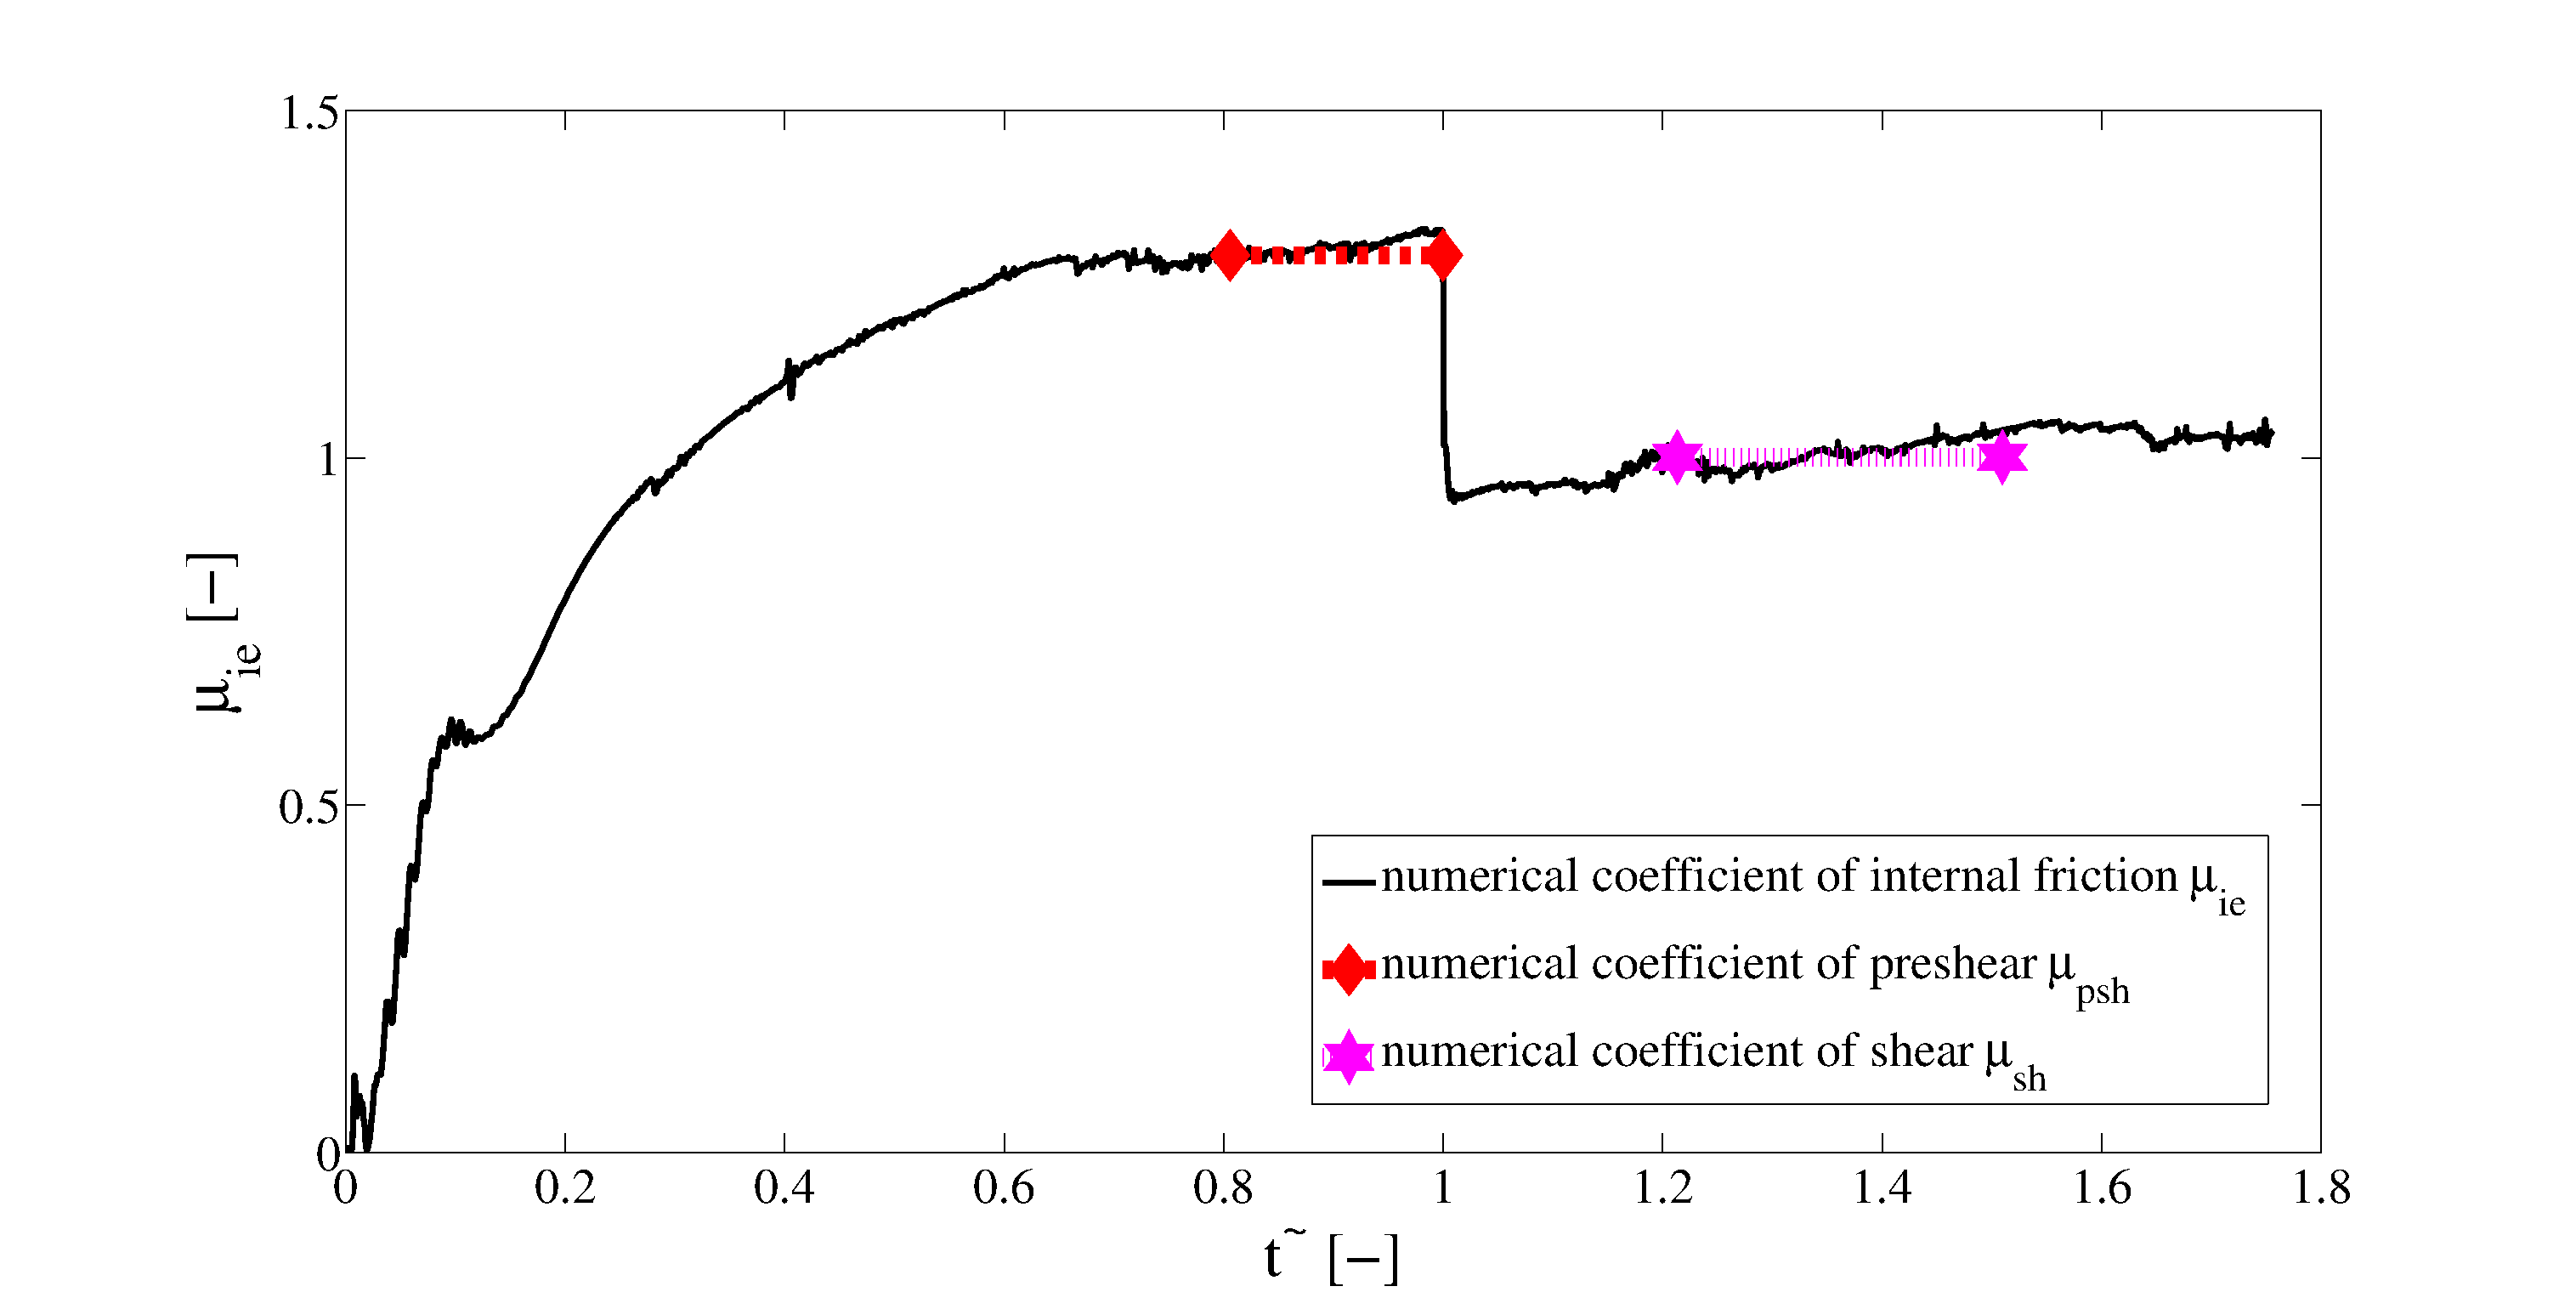
\includegraphics[width=\textwidth]{images/original/21simexample}
        \caption{Numerical shear cell tester stress path - $\sigma_n = 10000
        [Pa]$}
        \label{fig:21simexample} 
    \end{subfigure}
    \caption[Stress path]{Sample of the stress path for
	the Schulze ring shear cell tester, experimental and numerical.
	Time is normalized: $\tilde{t} = t/t_{change}$, where $t_{change}$ is the
	time when the normal stress ($\sigma_n$) is modified during the tests.
	Until $\tilde{t}=1$ the $\sigma_n = 2000 ~[Pa]$ is kept constant. 
	In Fig. \ref{fig:20experimental} at $\tilde{t}~=0.91$
 	a plateau is reached.
	The $\mu_{psh}$ is calculated as average of the $\mu_{ie}$ in this first
	plateau.
	Later, at $\tilde{t}=1$, the $\sigma_n$ is reduced to $80 \%$ of its initial
	value.
	Soon, a second plateau starts.
	As average of $\mu_{ie}$ in this second plateau we obtain $\mu_{sh}$.
	The stress path is in the numerical simulation is comparable to the
	experimental one, especially the plateaux.
	They were clearly relevant because there we collected the numerical bulk
	behaviour representative values. }
    \label{fig:40experimentalsimulation}
\end{figure}

\begin{table}[h]
\centering
\begin{tabular}{cccccc}
\hline
$\sigma_n$ (Pa) & $\tau$ (Pa) & $\mu_{psh}$ (-) & $\tau_{\%}$ (\%) &
$\mu_{sh}$ (-) & $\rho_b$ (kg/m3) \\
\hline
    1068  & 1059  & 0.9916 & 80 & 1.2333 & 1718 \\
    2069  & 1818  & 0.8787 & 80 & 0.9994 & 1759 \\
    10070 & 8232  & 0.8175 & 80 & 1.1712 & 1802 \\

\hline
\end{tabular}
\caption[Experimental results]{Experimental results. Values for three
load conditions}
\label{tab:05sinterTableExperimental}
\end{table}

\subsection{DEM Simulations}
\label{subsec:simulations}

For sinter fine 546 shear cell and 81 static angle of repose simulations have
been realized with the variations described in table
\ref{tab:10DEMVariableinputvalues}.
A representative stress path can be seen in Fig. \ref{fig:21simexample}.
Although the duration is smaller by two order of magnitude, the stress path is
comparable to the experimental one, especially the plateaux.
They were clearly relevant because there we collected the numerical bulk
behaviour representative values.\\
The computational time resulted in 1 hour with 32 AMD cores for a benchmark
shear cell simulation and 9 hours for a benchmark $AOR$ simulation, both with 50K particles. 
Simulations with large $dCylDp$ required a greater time amount (e.g. with 400K
particles about 12 hours for the shear cell). \\

\subsection{ANN model development}
\label{subsec:annmodeldev}

First, we controlled the regression of the bulk behaviour parameters, e.g. the
$\mu_{psh}$, see Fig. \ref{fig:22regression}, where the corresponding plot for
the $NN$ with the maximum $R^2$ in shown. Each circle represents one of the 546
simulations.
The plot presents a consistent agreement between the $DEM$ results distribution
(T in the legend) and the $NN$ regression (or fitting) line.
The linear relationship between the
training values have been evaluated in Table \ref{tab:06inputRelationshipTable}.
The clearest connections were between $\mu_s$ and $\mu_{psh}$, and
$\rho_p$ and $\rho_b$.
Instead, for $\mu_{sh}$ and $AOR$ the $\mu_r$ balanced the influence of the 
$\mu_s$, and further parameters were worthly correlated. \\
Then we observed how the $R^2$ changed with the different number of neurons for the $\mu_{psh}$. 
In this case we reached a $R^2 = 0.96$ for a $NN$ with fifteen neurons. 
Increasing the number of neurons did not improve the $R^2$, that even started to oscillate with the neuron number. 
Later, we processed the random combinations (table
\ref{tab:10DEMVariableinputvalues}) with the $NN$.
The $NN$ evaluation was incredibly faster compared to the $DEM$ simulations. The
individuation of all the marked $DEM$ combinations for the shear cell did not
take more than a few seconds on a single core.
We represented the marked combinations ($MC1$) for one load condition of the
shear cell ($\sigma_n=10070 ~[Pa]$, $P=1.0$) in Fig.
\ref{fig:24radarpirker1schulze10070}.
Here, the minimum and maximum values, together with the mean are shown. 
Furthermore, the shaded area represents valid parameters combinations.
Dark shaded values stand for the confidence range, provided by the square
deviation.
Notably, the confidence range is large, 
especially for the $COR$, highlighting its scarce influence over the characterization. 
Instead, both the $\rho_p$  and the $\mu_s$ show a narrow confidence range, 
displaying at the same time their influence and the validity of this procedure to find valid $DEM$ parameters. 
That agrees with the examination of the ratio of the standard deviation to the
range, see table \ref{tab:13DEMvalidvalues}.
Further, we could see how different $DEM$ parameters
combinations could reproduce the experimental behaviour and evaluate their mutual dependencies. 
This is clearer in a density plot, as in Fig. 
\ref{fig:25cloudpirker1schulze10070} for $MC1$, 
of the particles' coefficient of restitution (COR) in dependence
of coefficient of sliding friction and coefficient of rolling friction; in the
white area no valid sets of simulation parameter can be found.
In each cell the valid sets are grouped accordingly to the 4 different COR
ranges.
Each cell is colored accordingly to the group with the most members. 
While the $COR$ varied, multiple
combinations ($250407 --> 4\% $ of the total) of $\mu_s$ and $\mu_r$ reproduced
the experimental behaviour.
This underlines once more their correlation, as already stated by Wensrich and 
Katterfeld \cite{RefWorks:87}.
To further demonstrate the validity of the procedure, we modified the product
coefficient. In the first attempt we set it to $P=0.8$ and we obtained another
series of marked combinations ($MC2$).
We can see in the radar plot in Fig.
\ref{fig:26radarpirker08schulze10070} that the confidence range is narrower
compared to $P=1.0$, while in the density plot in Fig. 
\ref{fig:27cloudpirker08schulze10070} the area
appears larger, although slightly less densely populated. Finally, for $P=1.2$
and its marked combinations ($MC3$) the radar plot in Fig.
\ref{fig:28radarpirker12schulze10070} shows a largely different confidence
range, while the density plot in Fig. \ref{fig:30cloudpirker12schulze10070} 
illustrates a smaller area. As expected, the procedure was highly sensible to the variations of the experimental data. 
Thus, it could be effectively handled for a wide range of bulk materials.\\
We then processed the random combinations with the $AOR$ $NN$. In Fig.
\ref{fig:31radarpirker1aor} the radar plot realized with the same criteria as
before can be seen.
In accordance with the theory (Wensrich and Katterfeld \cite{RefWorks:87}), in a simulation dominated
by the particles rolling the coefficient of rolling friction has the maximum
influence. \\
Finally, we extracted from the $TC1$ values the $AOR$ $NN$ behaviour
and compared it with the experimental one.
As can be seen in the radar plot in Fig.
\ref{fig:33radarpirker1schulze10070aor}, the confidence range is meager, indicating that all the parameters but the $COR$ 
had an important role and the reliability of these parameters combinations to represent the bulk behaviour. 
From the initial 6250000 combinations, only 3884 of them were valid (0.0621 \%),
see table \ref{tab:13DEMvalidvalues}.
\begin{figure}%[!h] 
\centering 
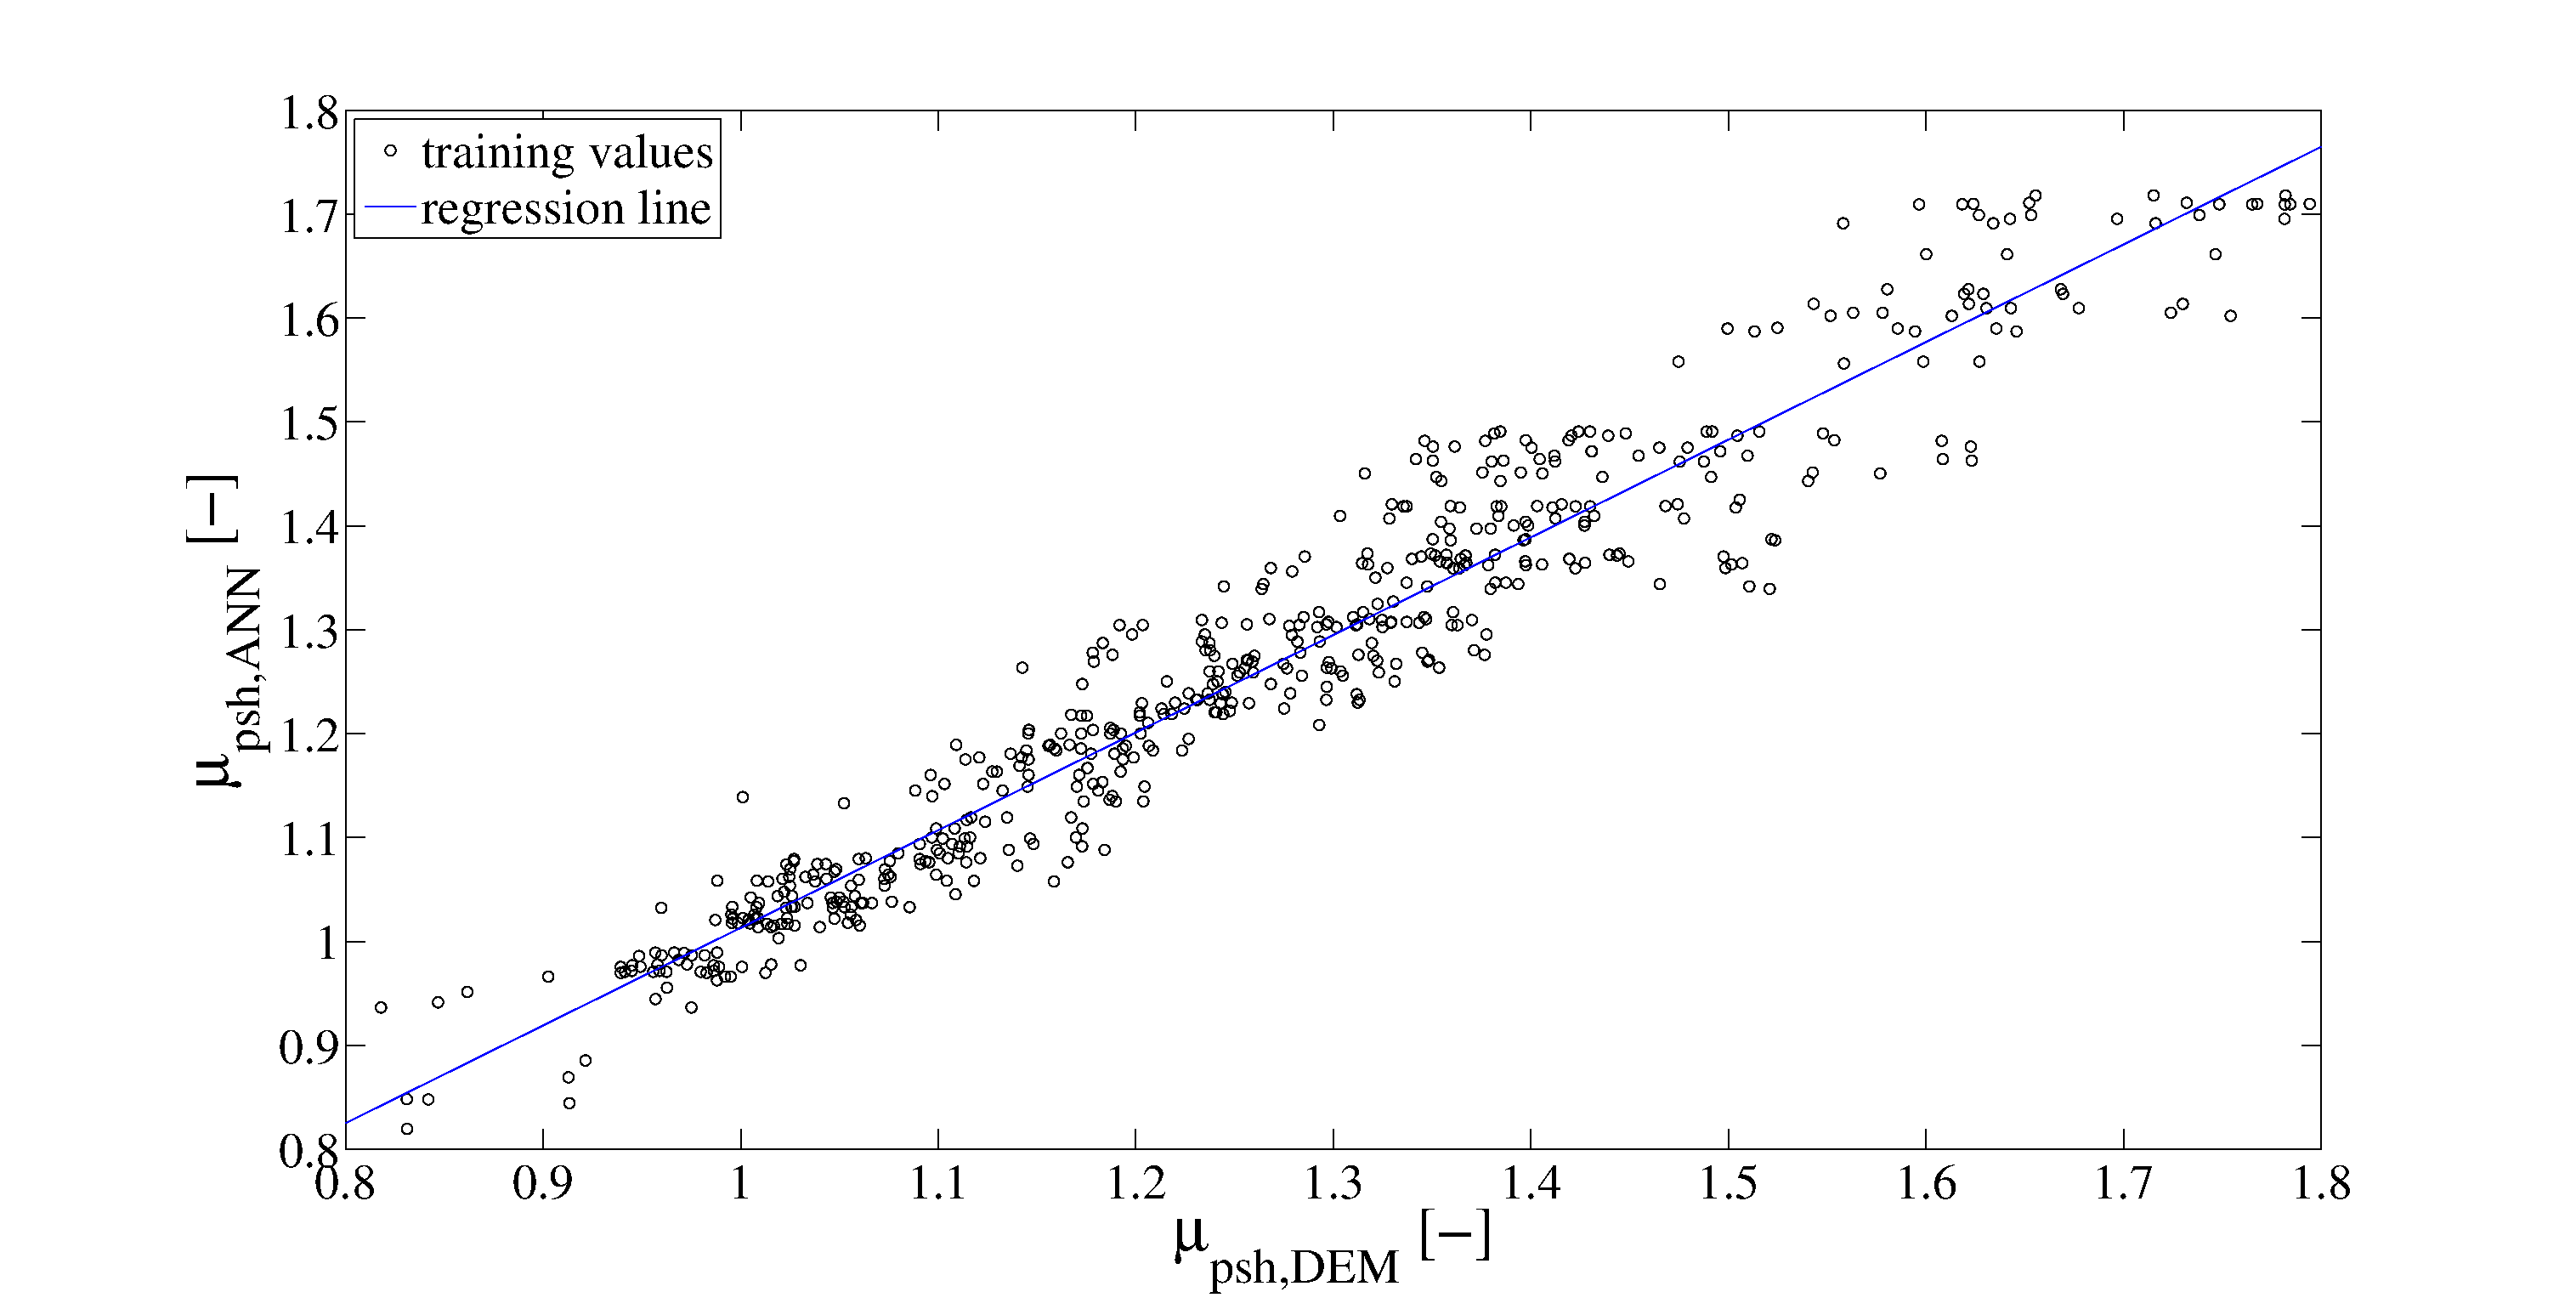
\includegraphics[width=.96\columnwidth]{images/22regression.eps}
%[width=.96\textwidth]
\caption[Comparison between prediction of the trained ANN and full DEM
simulation]{Comparison between prediction of the trained Artificial Neural
Network ($ANN$) and 546 
\wrong{write down all the simulations performed at the end.}
full DEM simulations of the coefficient of pre-shear
($\mu_{psh}$).}
\label{fig:22regression} 
\end{figure}
\begin{table}[h]
\centering
\scalebox{1.0}{
\begin{tabular}{c|cccccccc}
\hline
          & $\mu_s$ & $\mu_r$ & $COR$ & $\rho_p$ & $\mu_{sh}$ & $\mu_{psh}$ & $\rho_{b}$ & $AOR$ \\
          \hline
    $\mu_s$ & 100.00 & 0.55  & 0.04  & 0.00  & 3.84  & 87.26 & 8.39  & 49.48 \\
    $\mu_r$ & 0.55  & 100.00 & 0.15  & 0.00  & 58.92 & 33.70 & 3.10  & 60.20 \\
    $COR$ & 0.04  & 0.15  & 100.00 & 0.00  & 15.52 & 0.57  & 1.71  & 0.00 \\
    $\rho_p$ & 0.00  & 0.00  & 0.00  & 100.00 & 4.98  & 5.71  & 99.00 & 0.00 \\
    $\mu_{sh}$ & 3.84  & 58.92 & 15.52 & 4.98  & 100.00 & 26.03 & 9.52  & 0.00 \\
    $\mu_{psh}$ & \textbf{87.26} & 33.70 & 0.57  & 5.71  & 26.03 & 100.00 & 4.33 
    & 0.00
    \\
    $\rho_{b}$ & 8.39  & 3.10  & 1.71  & \textbf{99.00} & 9.52  & 4.33  & 100.00
    & 0.00 \\
    $AOR$ & 49.48 & \textbf{60.20} & 0.00  & 0.00  & 0.00  & 0.00  & 0.00  &
    100.00 \\
    
\hline
\end{tabular}}
\caption{Values of linear relationship between considered variables multiplied
for 100}
\label{tab:06inputRelationshipTable}
\end{table}
\begin{table}[h]
\centering
\begin{tabular}{llccc}
\hline

          & type  & SSC & AoR   & SSC \& AoR \\
          \hline

    $\mu_s$ & mean  & 0.831 & 0.177 & 0.664 \\
    $[-]$   & std. dev. (SD) & 0.097 & 0.095 & 0.029 \\
          & range ($R$) & 0.9   & 0.9   & 0.9 \\
          & SD / R & 0.108 & 0.106 & 0.032 \\
          \hline
    $\mu_r$ & mean  & 0.692 & 0.830 & 0.916 \\
    $[-]$   & std. dev. (SD) & 0.215 & 0.193 & 0.042 \\
          & range ($R$) & 0.9   & 0.9   & 0.9 \\
          & SD / R & 0.239 & 0.214 & 0.046 \\
          \hline
              COR   & mean  & 0.708 & 0.590 & 0.590 \\
   $ [-]$   & std. dev. (SD) & 0.104 & 0.073 & 0.065 \\
          & range ($R$) & 0.4   & 0.4   & 0.4 \\
          & SD / R & 0.259 & 0.183 & 0.161 \\
          \hline
    $\rho_p$ & mean  & 2245.7 & 3192.8 & 2283.9 \\
    $[kg/m3]$ & std. dev. (SD) & 80.5  & 277.4 & 67.1 \\
          & range ($R$) & 1500  & 1500  & 1500 \\
          & SD / R & 0.054 & 0.185 & 0.045 \\
          \hline
    valid & number & 290203 & 816552 & 3884 \\
    combinations & [$\%$] & 4.64  & 13.06 & 0.06 \\  

\hline
\end{tabular}
\caption[DEM valid values]{DEM valid values. For each parameter we show the
valid parameters statistics in the two tests and in their intersection.
Finally, we show the number of valid parameters combinations over the total
(6250000).}
\label{tab:13DEMvalidvalues}
\end{table}
\begin{figure}[htp] \centering
    \begin{subfigure}
        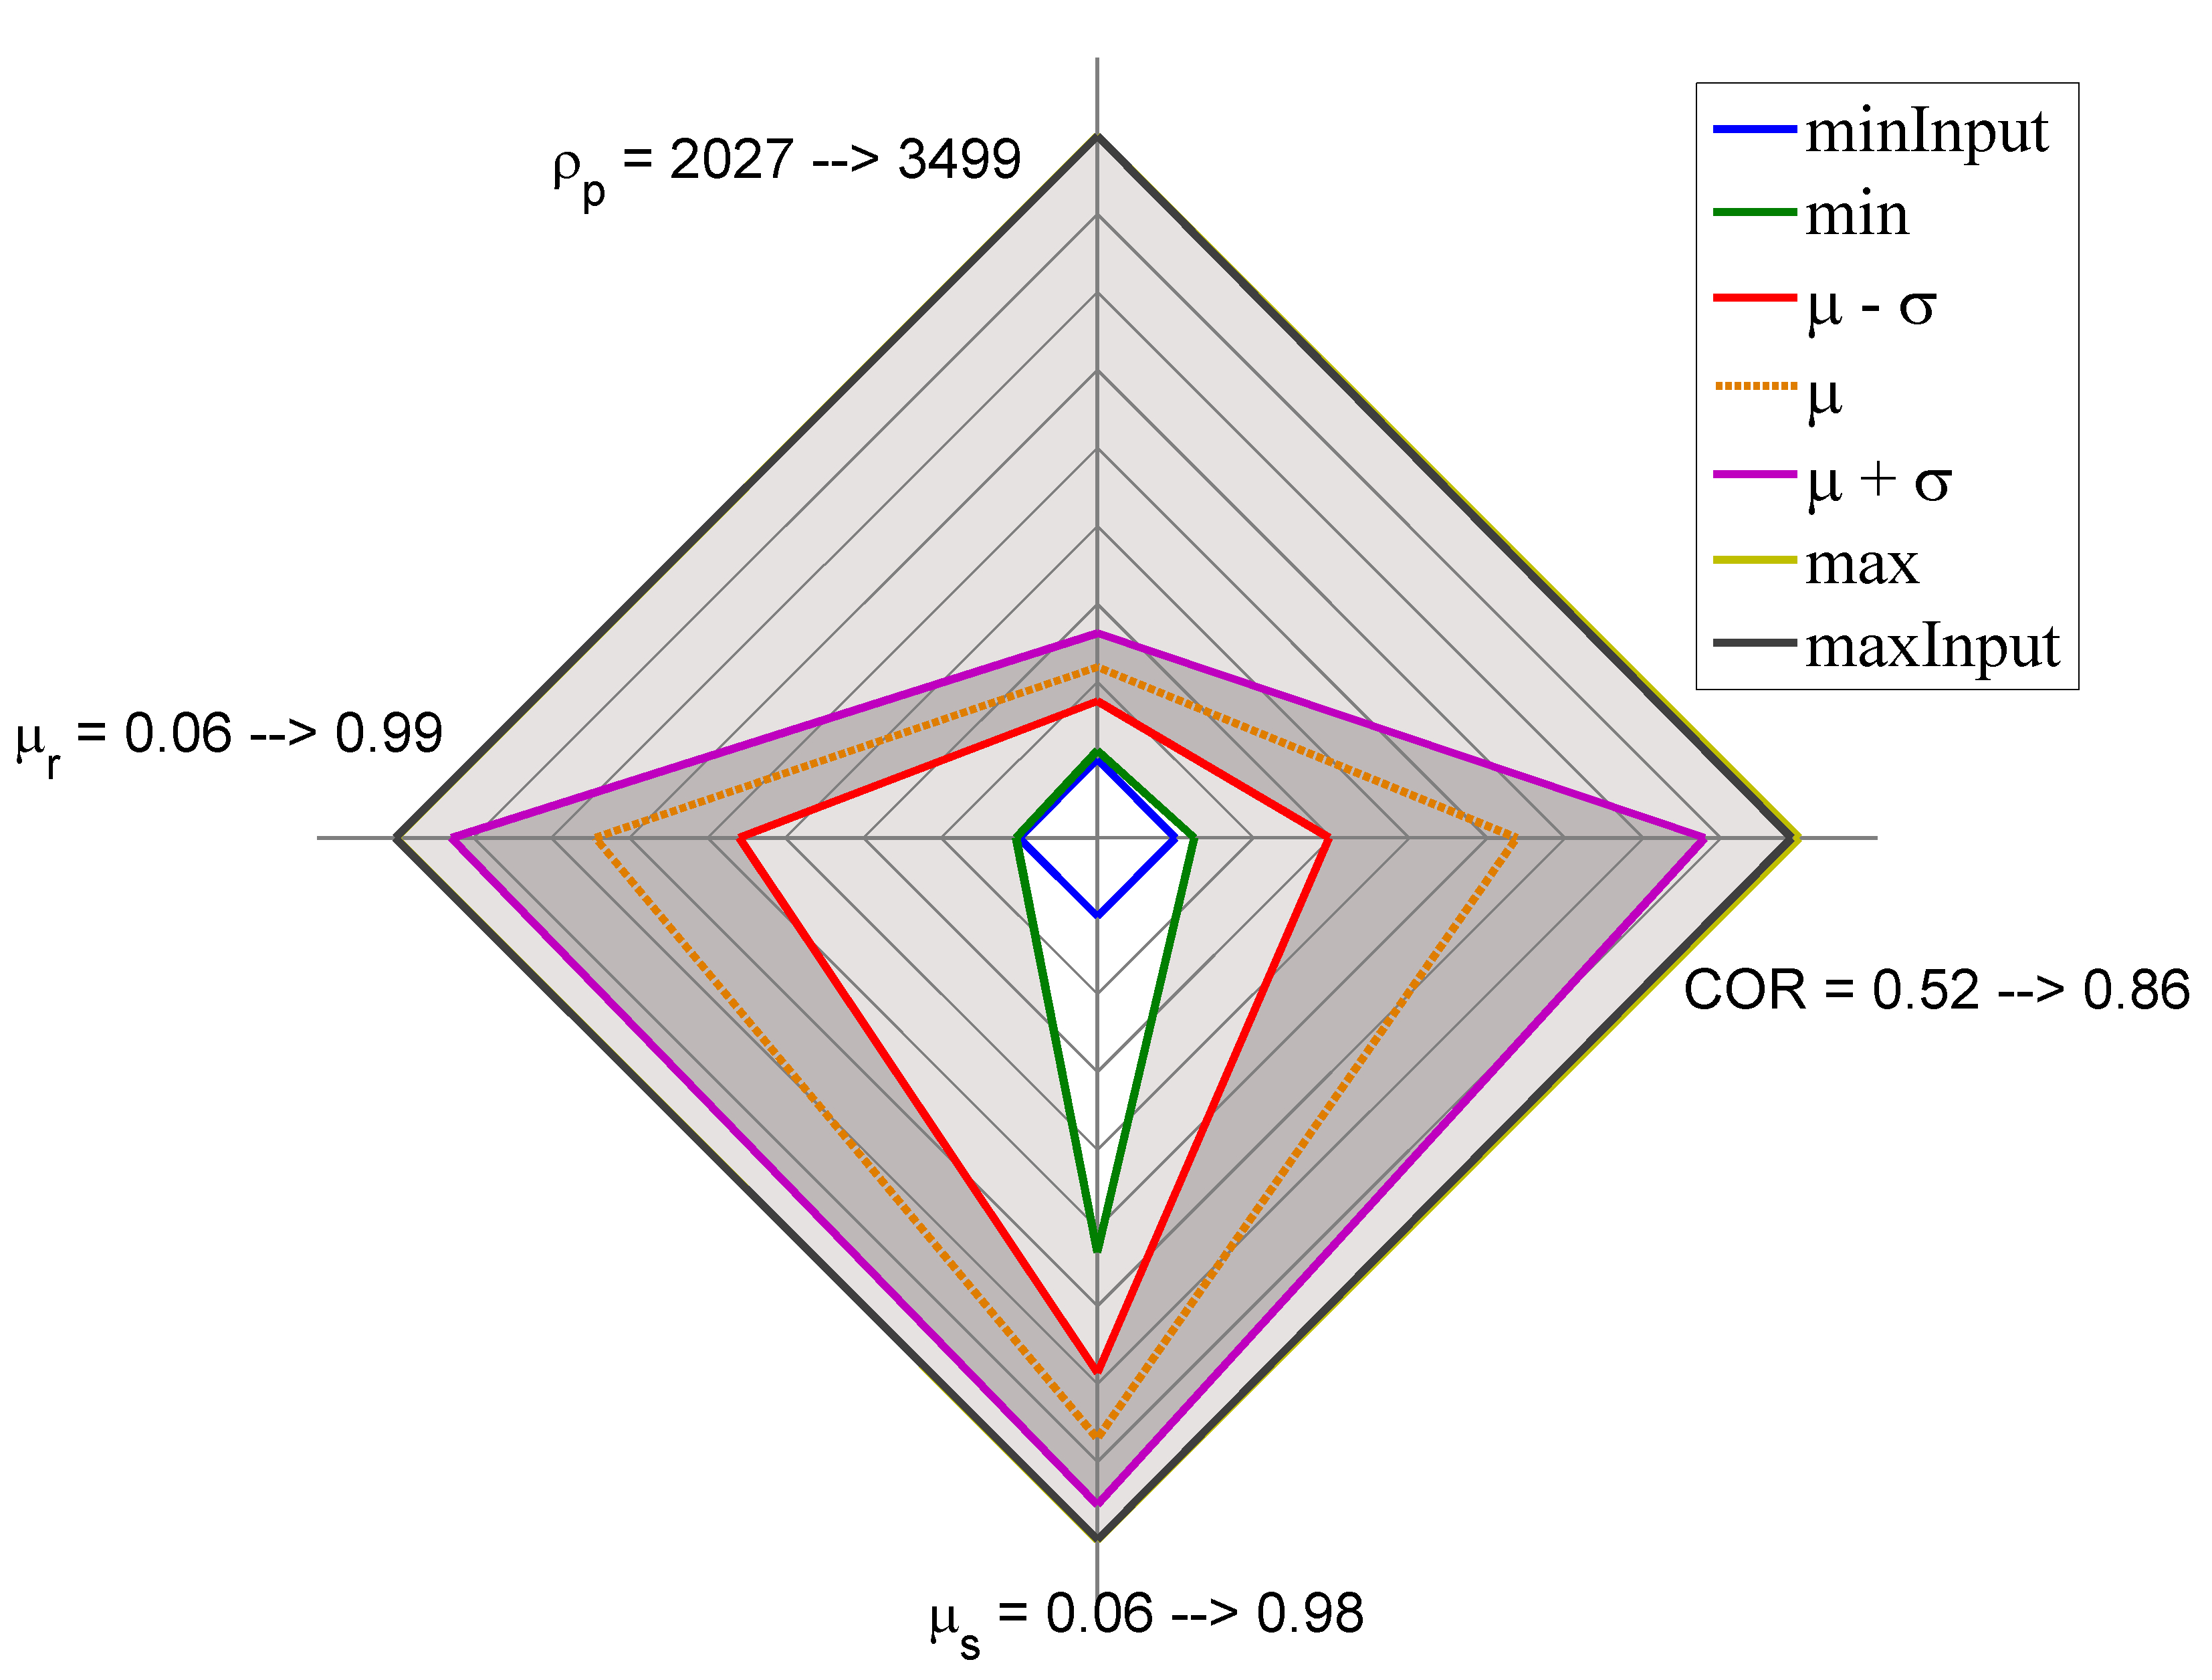
\includegraphics[width=0.5\textwidth]{images/original/24radarpirker1schulze10070}
        \caption{Radar plot, $SCT$, $\sigma_n=10070 ~[Pa]$, $P=1.0$}
        \label{fig:24radarpirker1schulze10070}
    \end{subfigure} \\
        \begin{subfigure}
        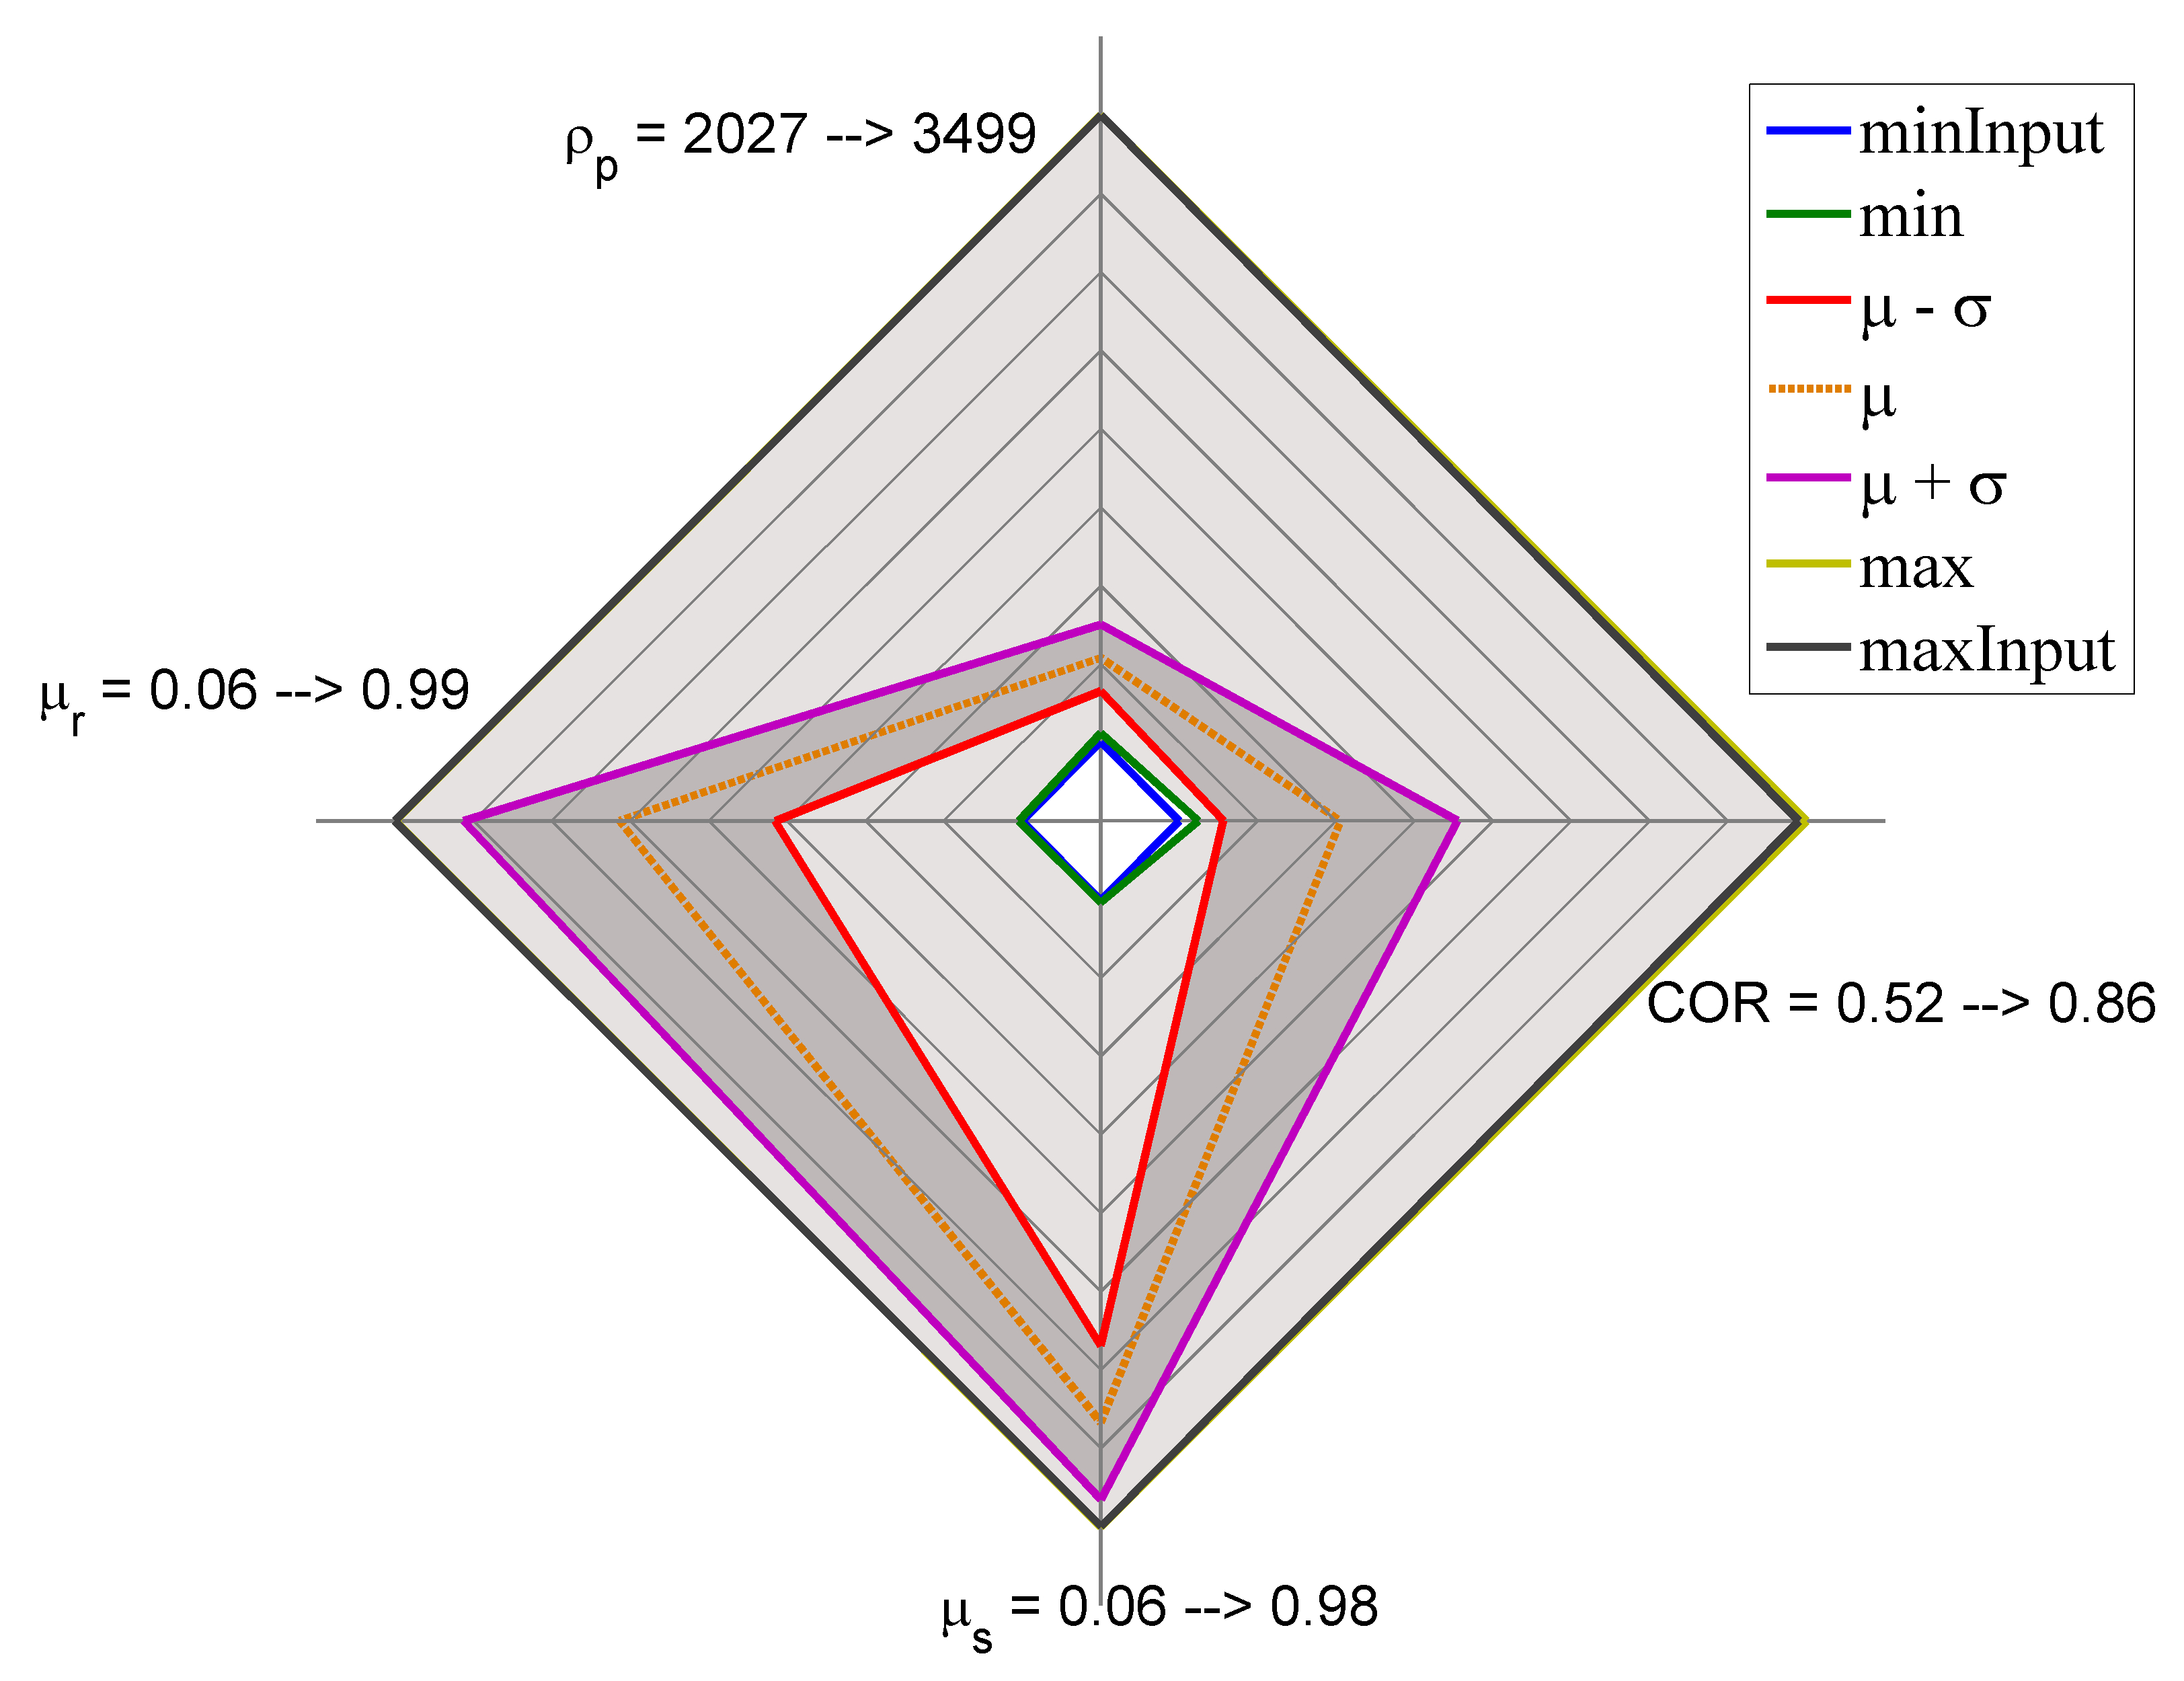
\includegraphics[width=0.5\columnwidth]{images/original/26radarpirker08schulze10070}
        \caption{Radar plot, $SCT$, $\sigma_n=10070 ~[Pa]$, $P=0.8$}
        \label{fig:26radarpirker08schulze10070} 
    \end{subfigure}\\
        \begin{subfigure}
        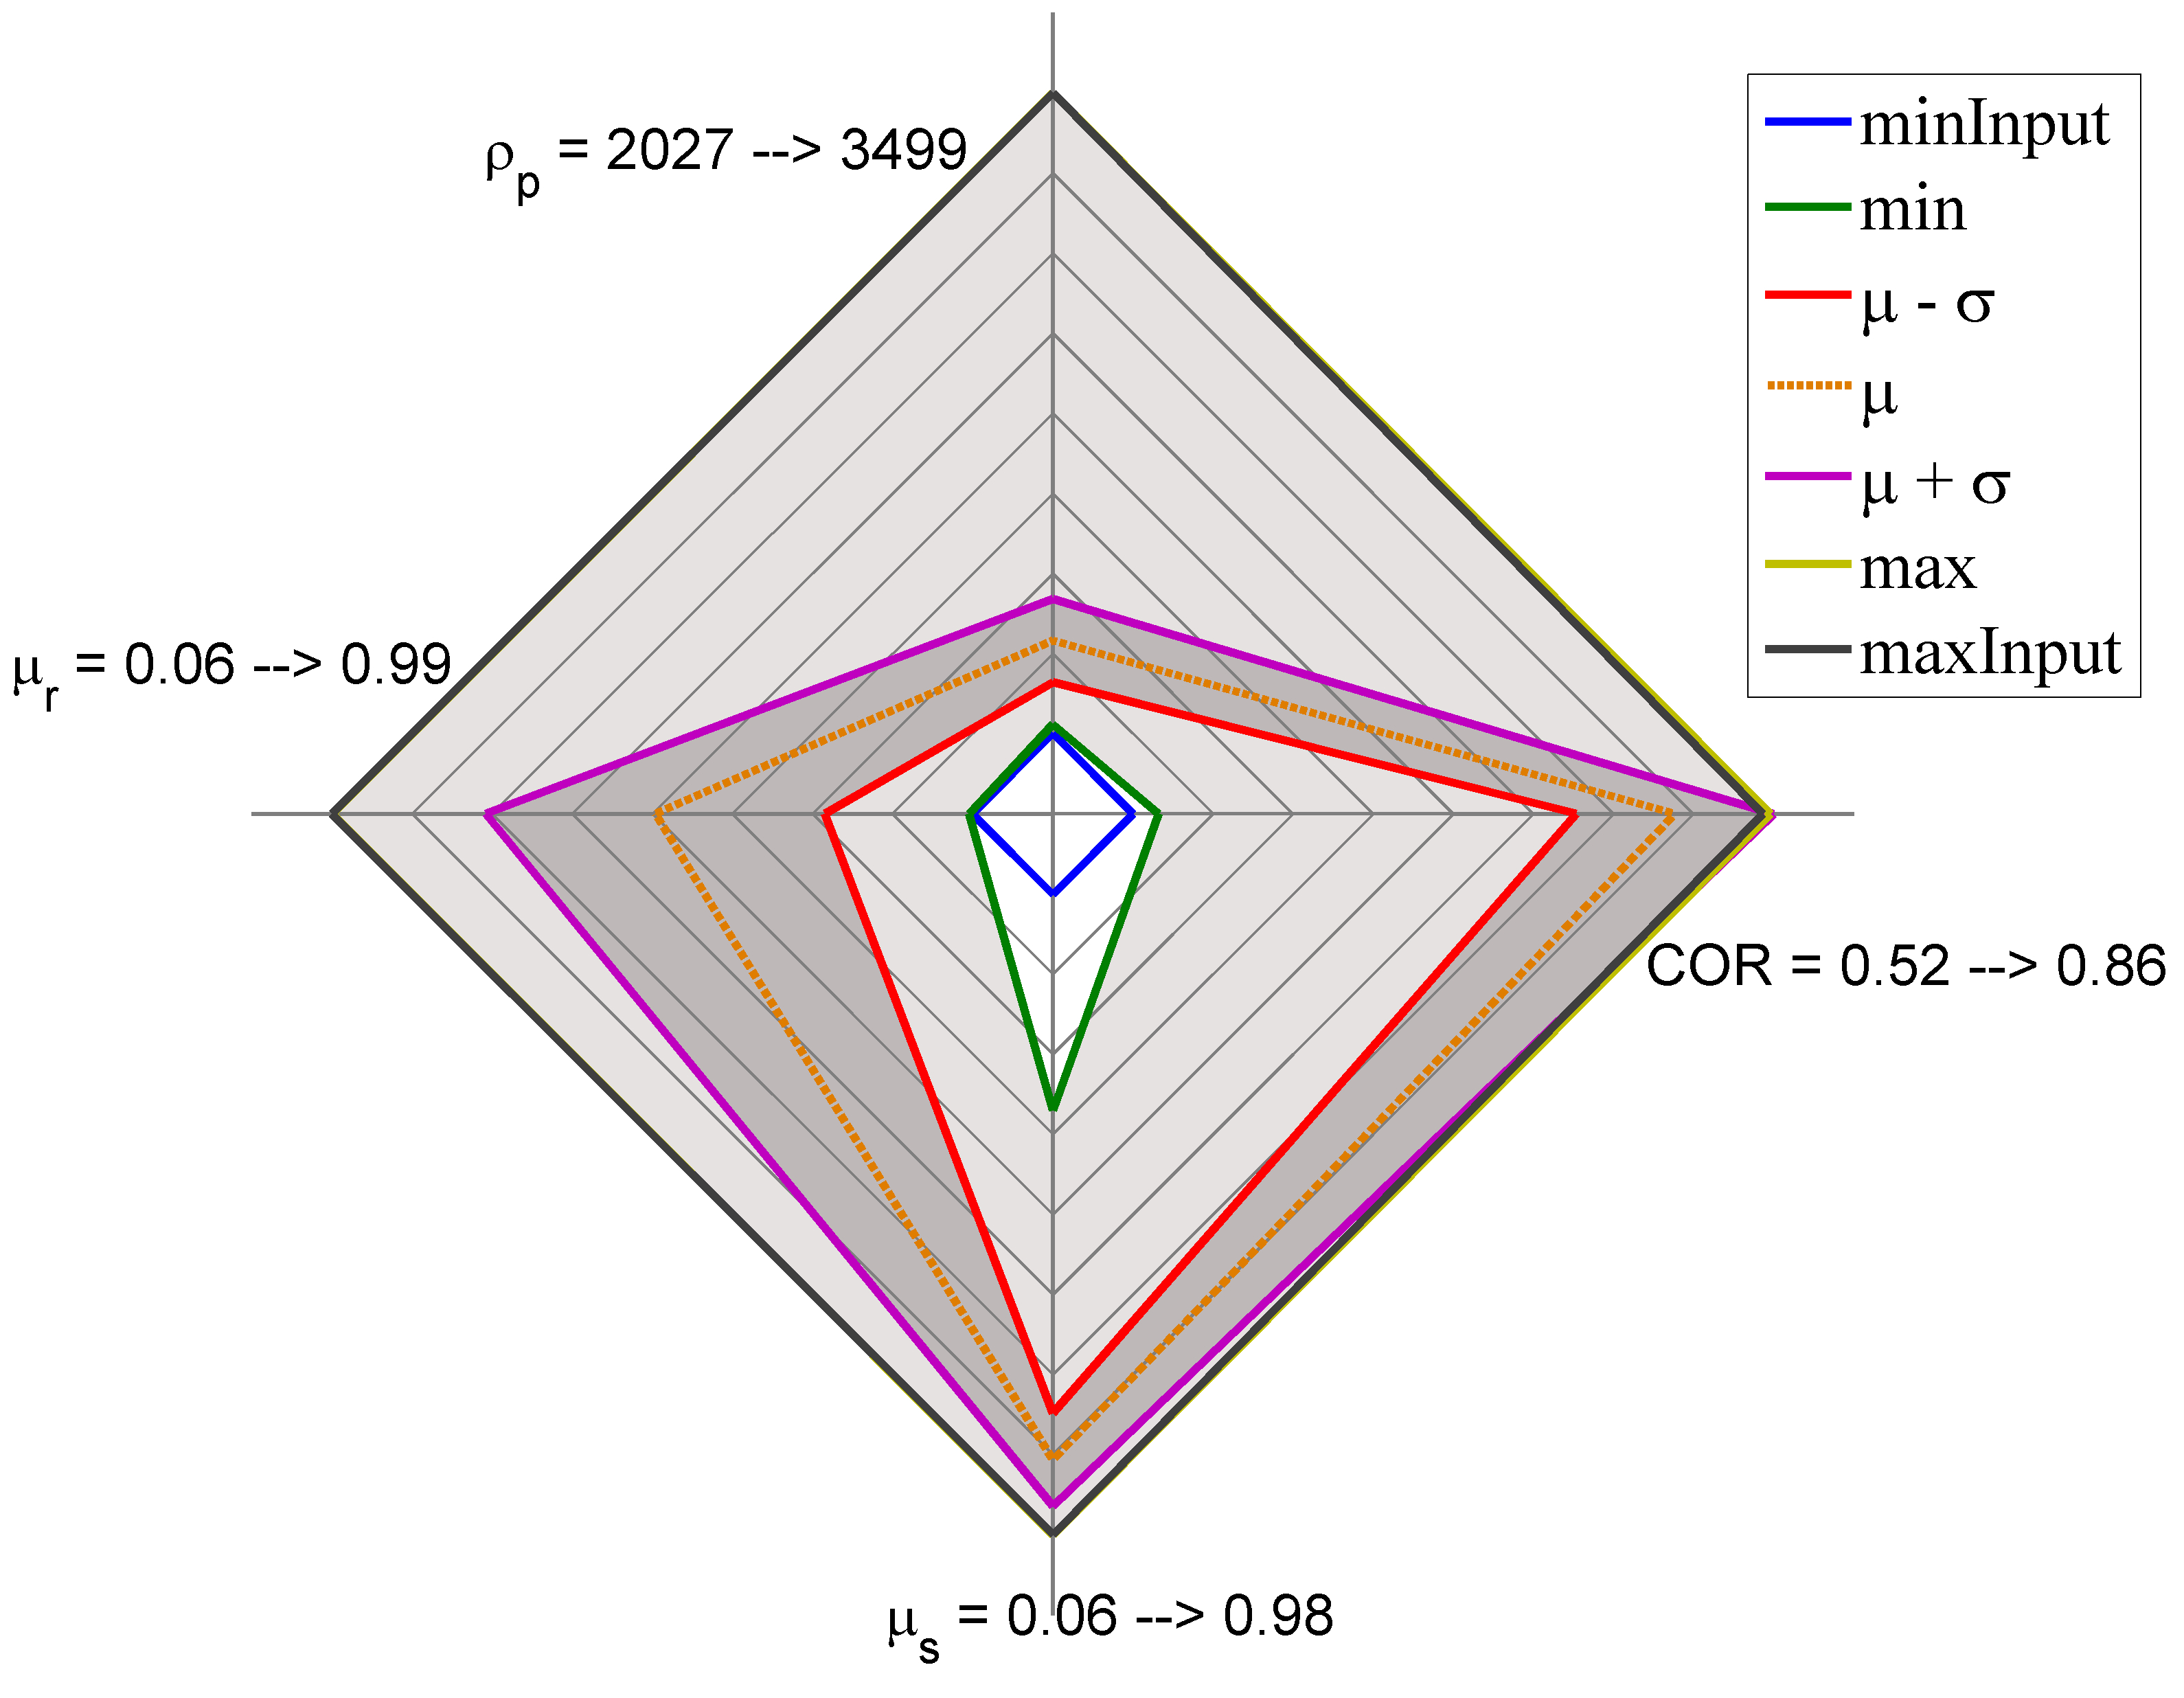
\includegraphics[width=0.5\columnwidth]{images/original/28radarpirker12schulze10070}
        \caption{Radar plot, $SCT$, $\sigma_n=10070 ~[Pa]$, $P=1.2$}
        \label{fig:28radarpirker12schulze10070} 
    \end{subfigure}
    \caption[Radar plot of valid simulations parameters for three different
    bulk behaviours measured by SCT]{Radar plot of valid simulations parameters for three different
    bulk behaviours measured by shear cell tester ($SCT$).
    Each axes of the radar plot represents one simulation parameters.
    Furthermore, the shaded area represents valid parameters combinations.
    Dark shaded values stand for the confidence range.
    We represent the tabbed combinations for one load condition of the shear cell. 
    Further explanation in the text.
   }
    \label{fig:29schulzeradarandcloud}
\end{figure}
% 
% The minimum and maximum values, together with the mean and the confidence range,
% provided by the square deviation, are shown.
%     Here, the values plotted are selected between the numerical
%     values from the $NN$ with initially the original experimental results for the shear cell tester $P=1.0$ (Fig.
%     \ref{fig:24radarpirker1schulze10070}). 
%     The confidence range is large, especially for the $COR$.
%     Instead, both the $\rho_p$  and the $\mu_s$ show a narrow confidence range. 
%     Later, they have been chosen with  
%     the virtual decreased results $P=0.8$
%     (\ref{fig:26radarpirker08schulze10070}).
%     The confidence range is narrower compared to $P=1.0$
%     The last image (Fig. \ref{fig:28radarpirker12schulze10070}) represents
%     instead the selection with the the virtual increased results $P=1.2$.
%     The plot shows a largely different confidence range. 
\begin{figure}[htp] \centering

    \begin{subfigure}[b]{0.96\columnwidth}
        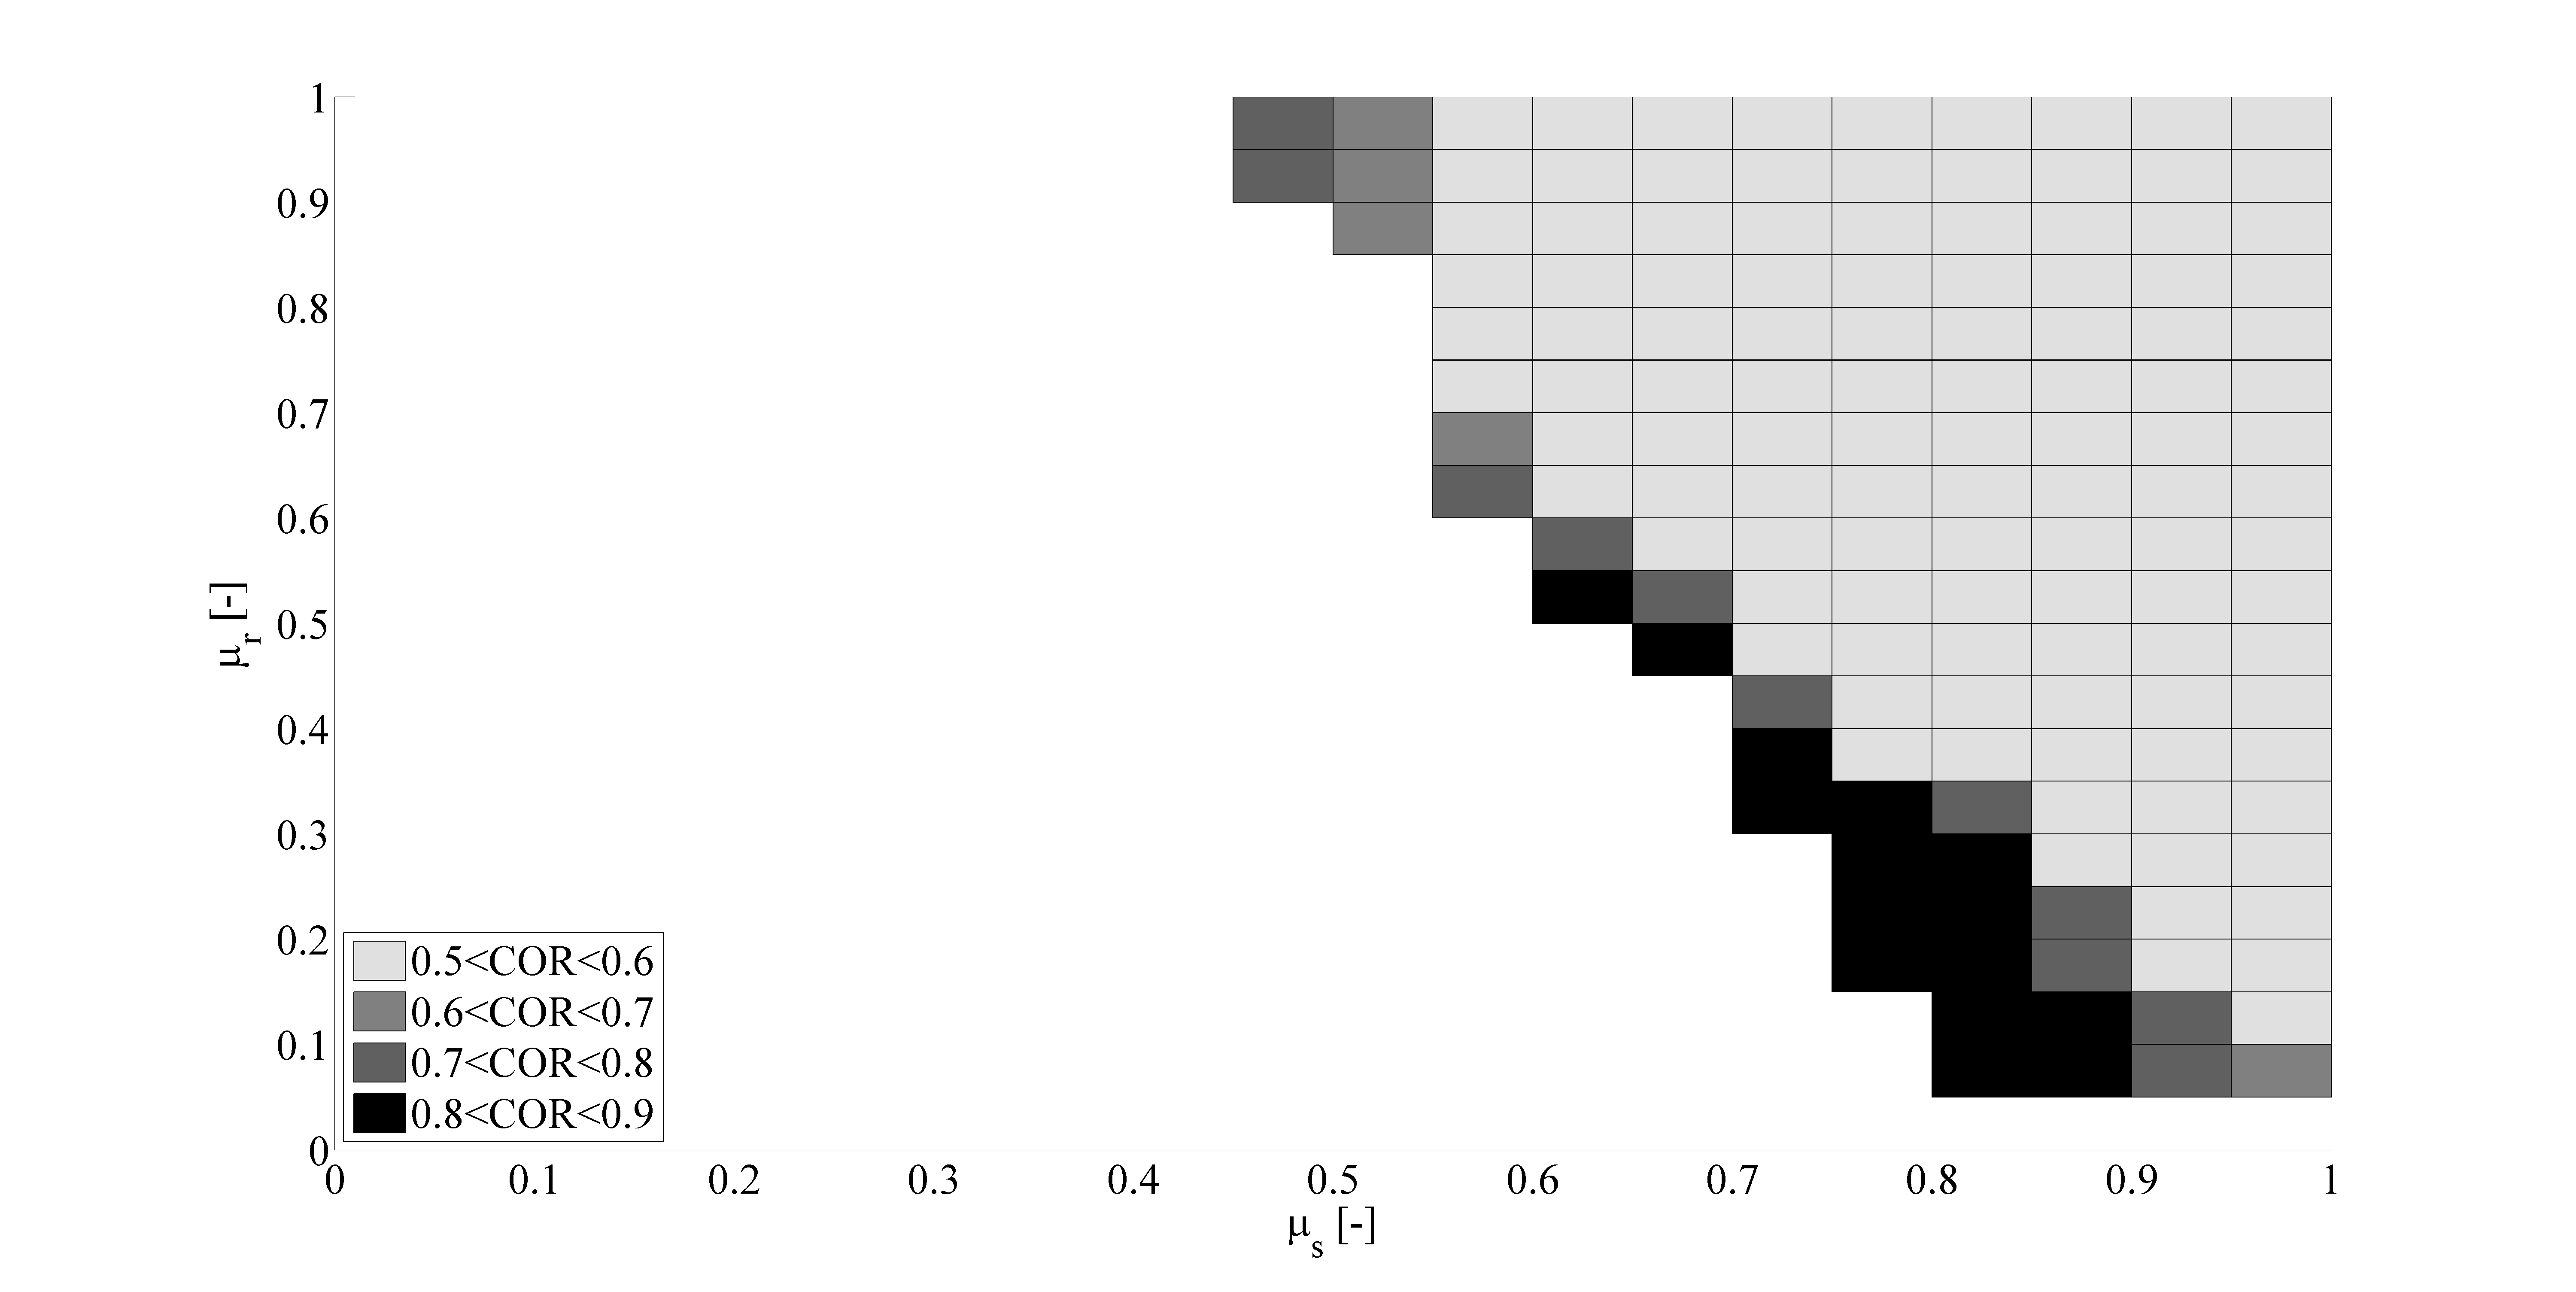
\includegraphics[width=\textwidth]{27cloudpirker08schulze10070}
        \caption{Cloud plot, $SSC$, $\sigma_n=10070 ~[Pa]$, $P=0.8$}
        \label{fig:27cloudpirker08schulze10070} 
    \end{subfigure}\\
    \begin{subfigure}[b]{0.96\columnwidth}
        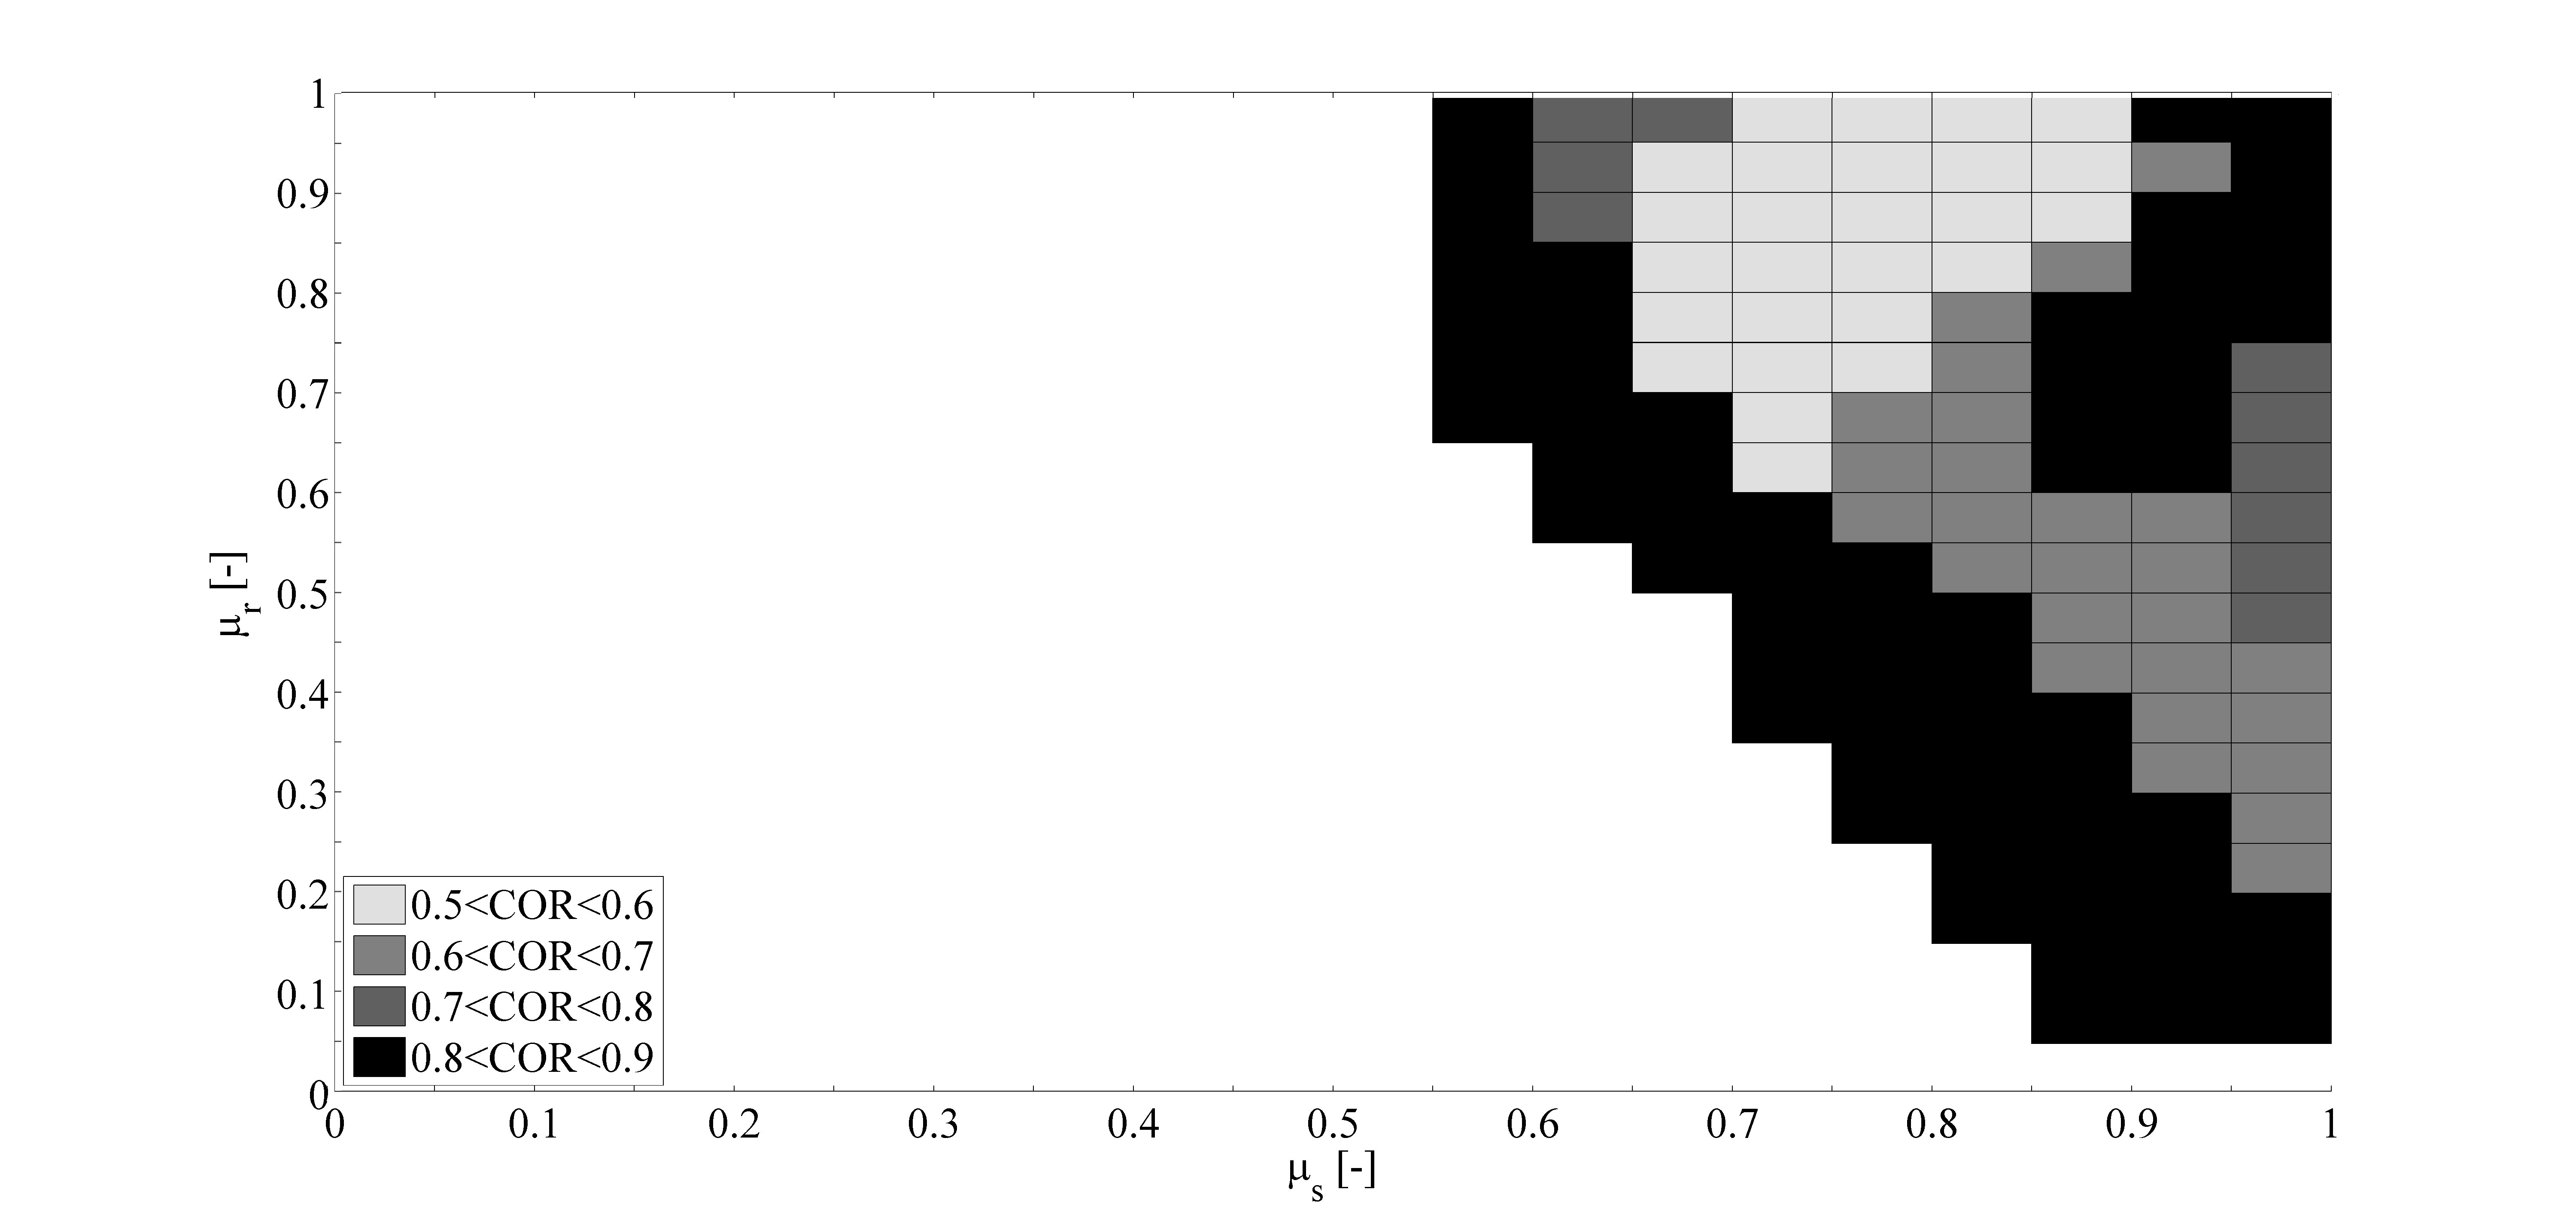
\includegraphics[width=\textwidth]{25cloudpirker1schulze10070}
        \caption{Cloud plot, $SSC$, $\sigma_n=10070 ~[Pa]$, $P=1.0$}
        \label{fig:25cloudpirker1schulze10070}
    \end{subfigure}\\

    \begin{subfigure}[b]{0.96\columnwidth}
        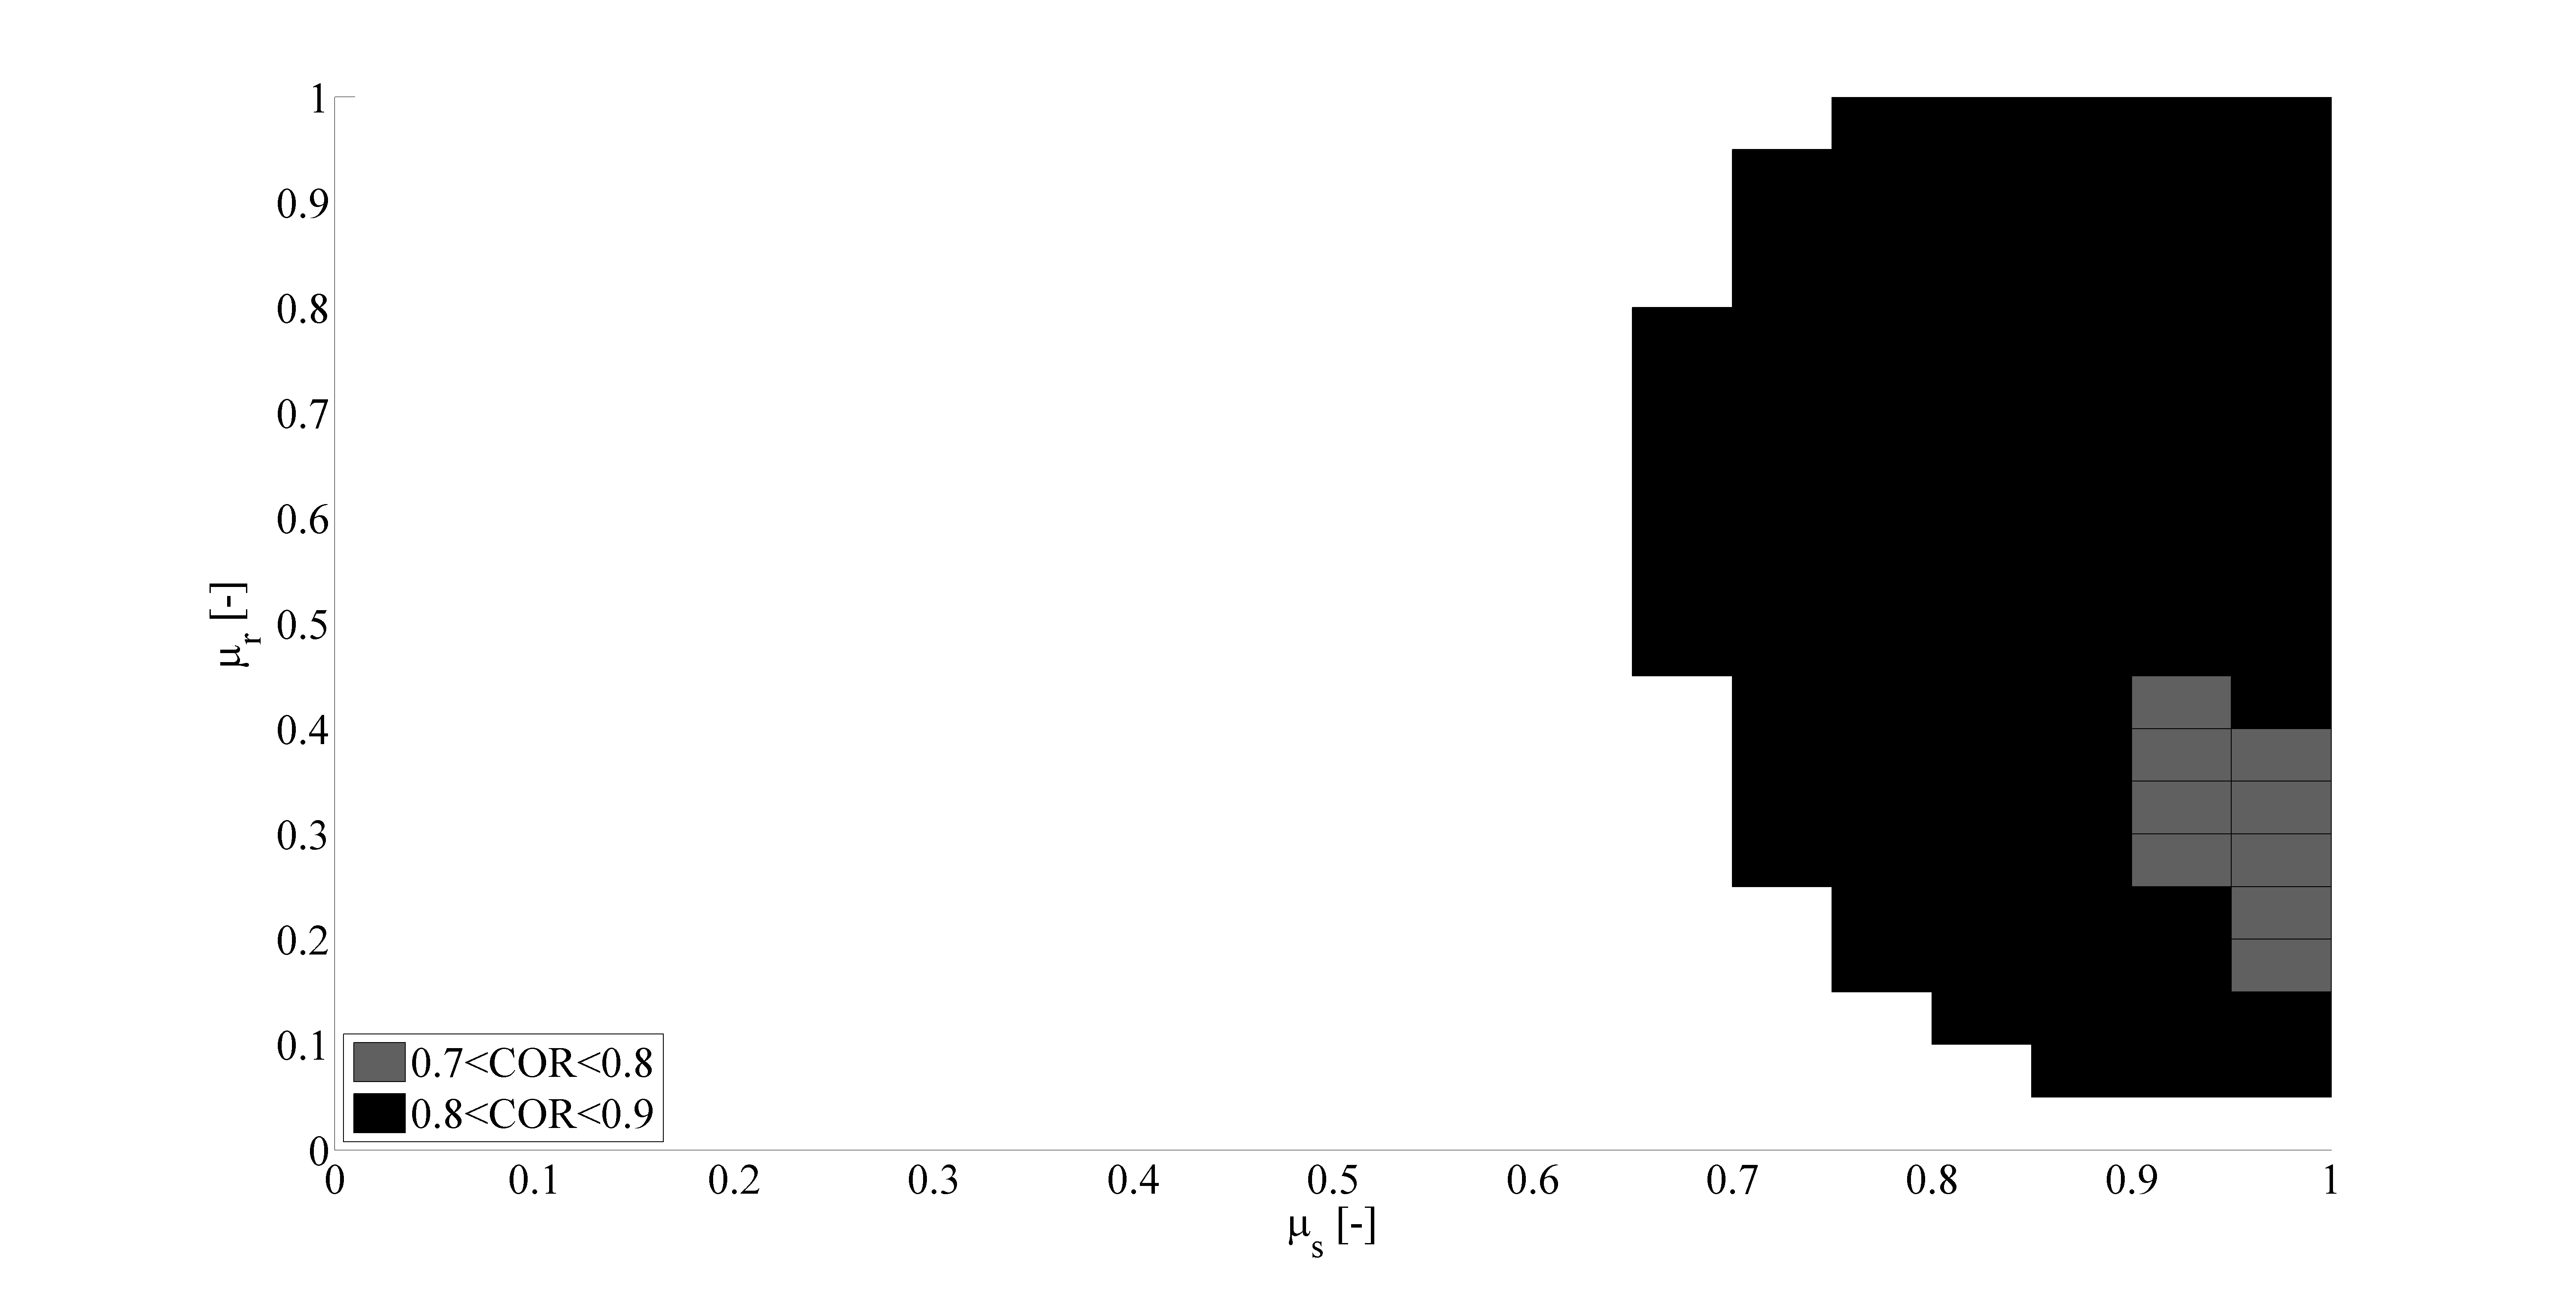
\includegraphics[width=\textwidth]{30cloudpirker12schulze10070}
        \caption{Cloud plot, $SSC$, $\sigma_n=10070 ~[Pa]$, $P=1.2$}
        \label{fig:30cloudpirker12schulze10070} 
    \end{subfigure}
    \caption[Density plot comparison of SCT results]{Density plot comparison of
    shear cell tester ($SSC$) results. We represent the marked combinations for
    one load condition of the shear cell. 
    Density plot of the particles' coefficient of restitution (COR) in dependence
	of coefficient of sliding friction and coefficient of rolling friction; in the
	white area no valid sets of simulation parameter can be found.
	In each cell the valid sets are grouped accordingly to the 4 different COR
	ranges.
	Each cell is colored accordingly to the group with the most members. 
    Here, the values plotted are selected between the numerical
    values from the Neural Network with initially the original experimental
    results for the $SSC$, with a product coefficient $P=1.0$ (Fig.
    \ref{fig:25cloudpirker1schulze10070}). 
        Later, they have been chosen with  
    the virtual decreased results $P=0.8$
    (\ref{fig:27cloudpirker08schulze10070}).
    The last image (Fig. \ref{fig:30cloudpirker12schulze10070}) represents
    instead the selection with the the virtual increased results $P=1.2$.    }
    \label{fig:29schulzeradarandcloud}
\end{figure}
\begin{figure}[htp] \centering
    \begin{subfigure}[b]{0.96\columnwidth}
        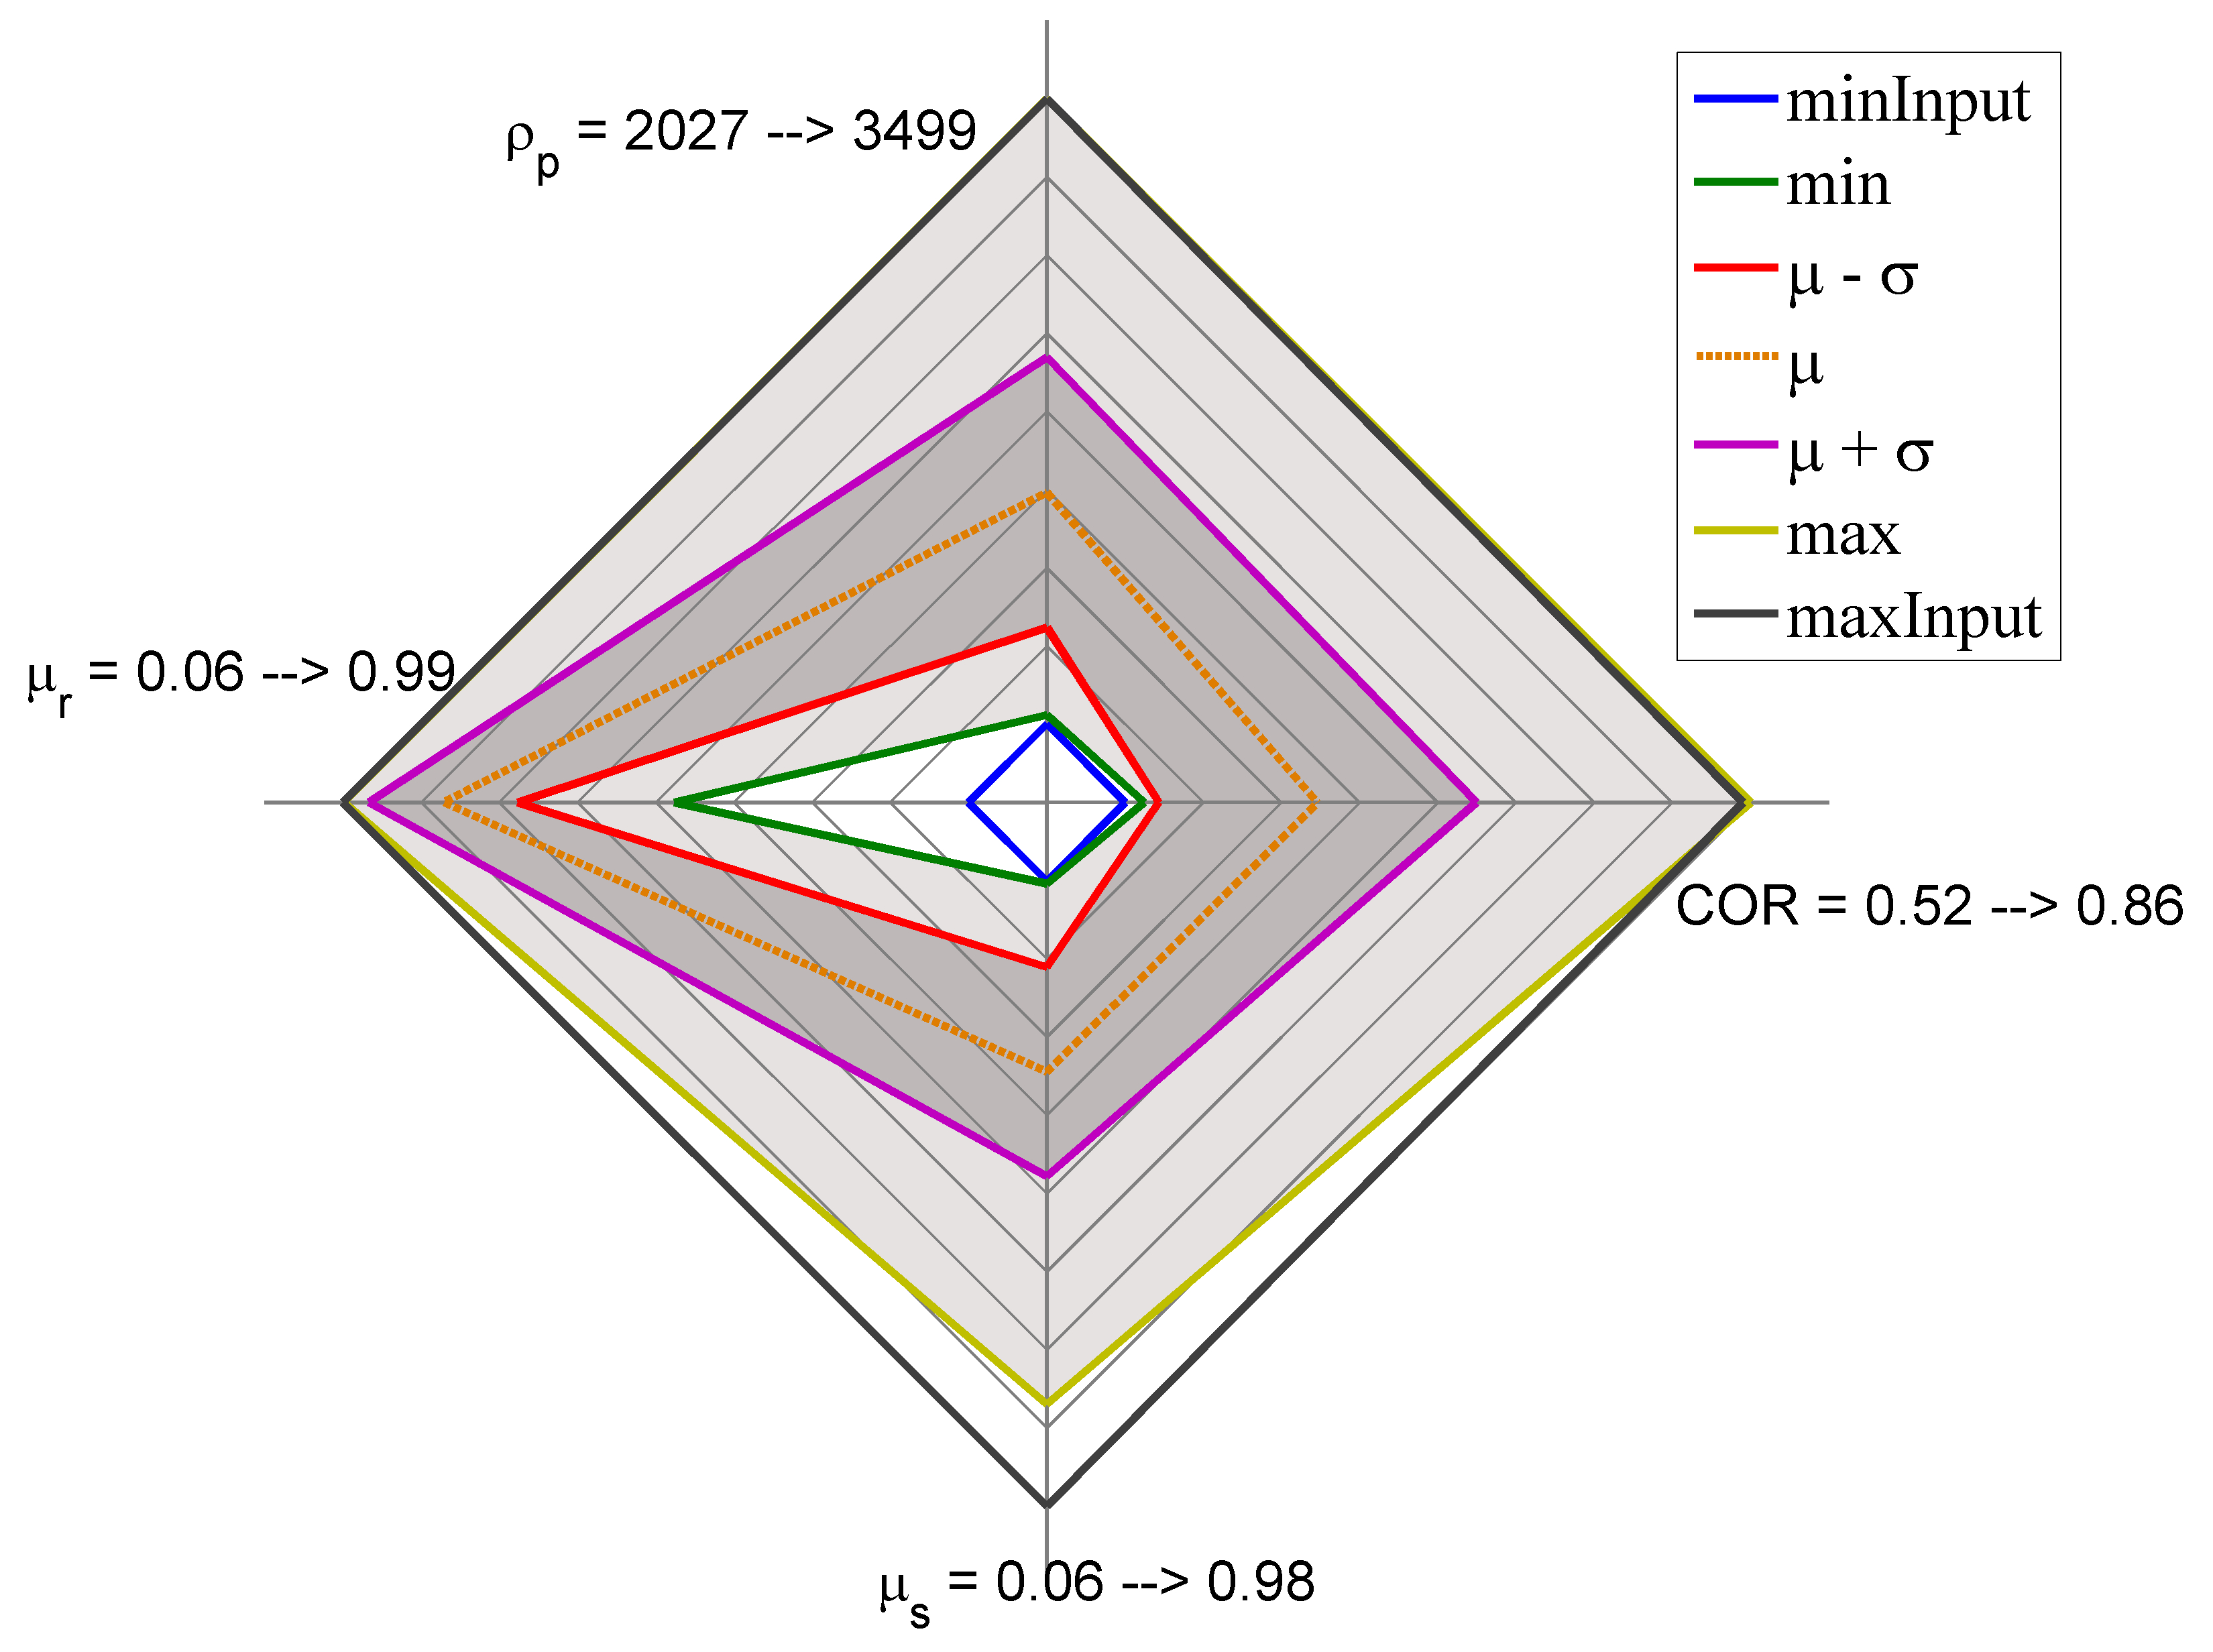
\includegraphics[width=\textwidth]{images/original/31radarpirker1aor}
        \caption{Radar plot, $AOR_{exp} = 38.85 ^\circ$}
        \label{fig:31radarpirker1aor} 
    \end{subfigure}\\
        \begin{subfigure}[b]{0.96\columnwidth}
        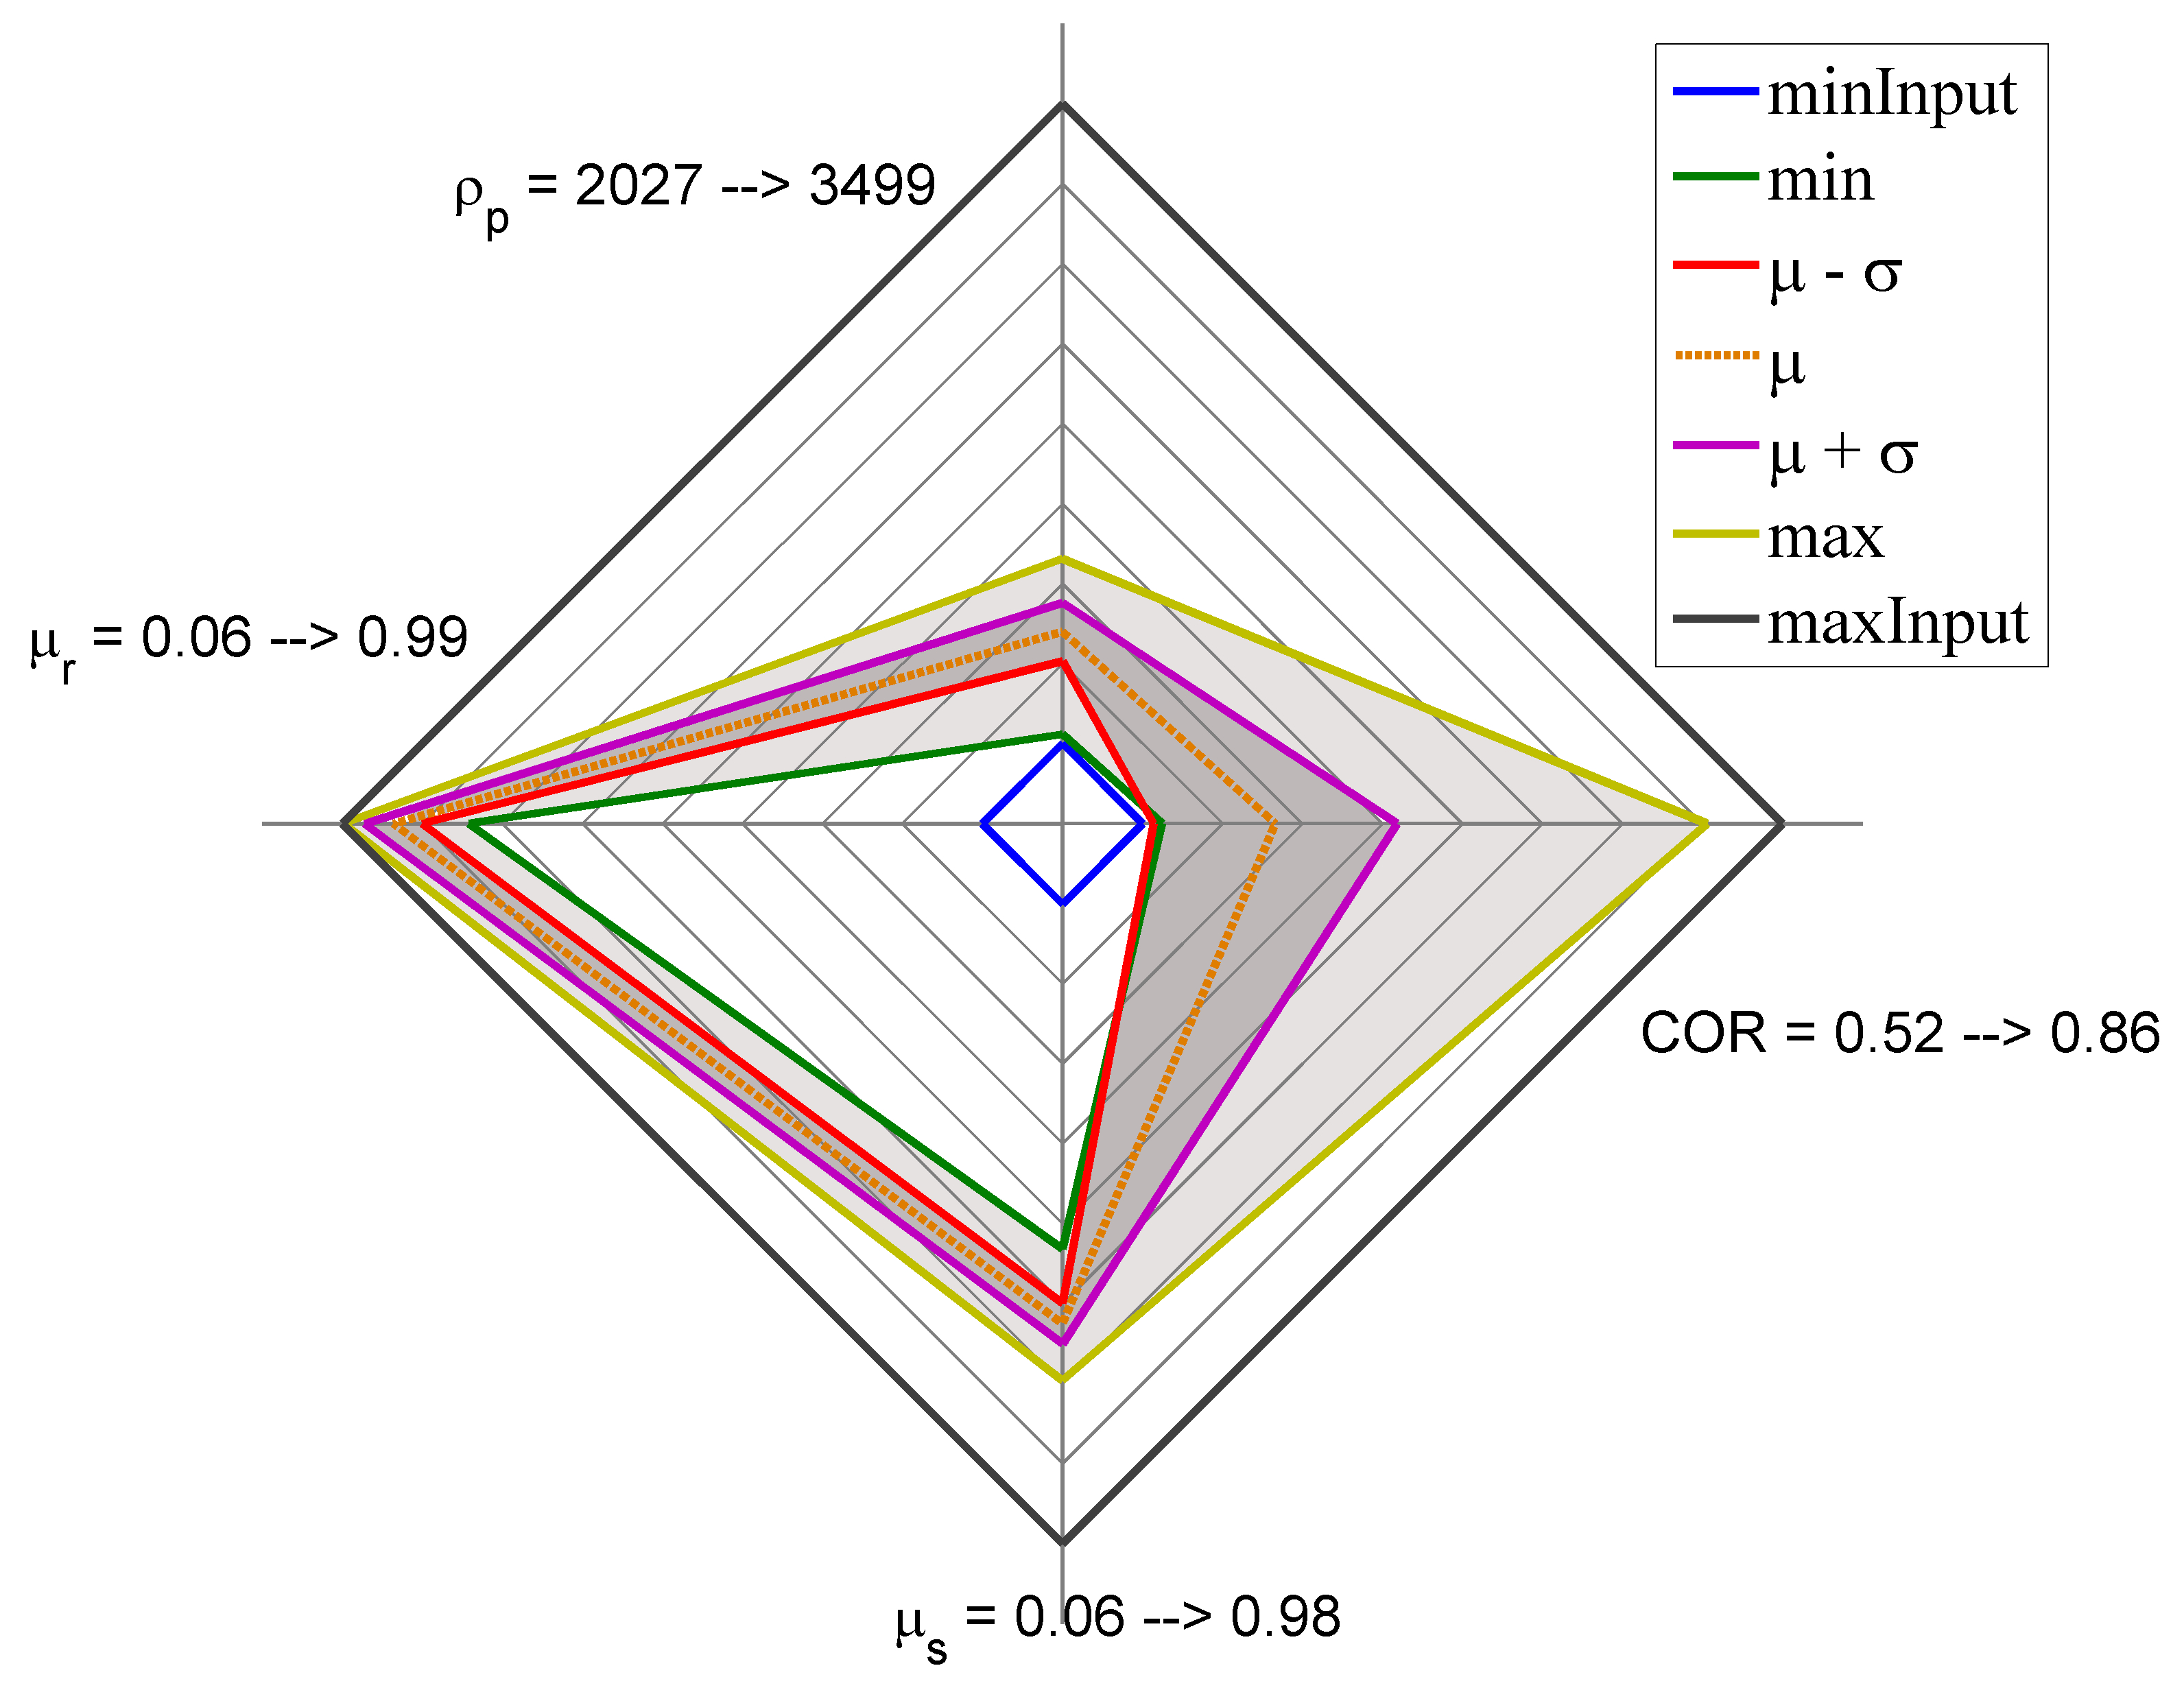
\includegraphics[width=\textwidth]{images/original/33radarpirker1schulze10070aor}
        \caption{Radar plot, $AOR_{exp} = 38.85
        ^\circ$, $SCT$, $\sigma_n=10070 ~[Pa]$}
        \label{fig:33radarpirker1schulze10070aor} 
    \end{subfigure}
    \caption[Radar plot comparison of AOR and SCT results]{Radar plot comparison
    of $AOR$ and $SCT$ results. We represent the tabbed combinations for the
    $AOR$ test.
    The minimum and maximum values, together with the mean and the confidence
	range, provided by the square deviation, are shown.
    Here, the values plotted are selected between the numerical
    values from the $NN$ with initially the original experimental results for
    the $AOR$, $P=1.0$ (Fig.
    \ref{fig:31radarpirker1aor}). 
    The confidence range is large, except for the $\mu_r$.
    The last image (Fig. \ref{fig:33radarpirker1schulze10070aor}) represents
    instead the values valid for both the $AOR$ test and the $SCT$, with a
    $\sigma_n=10070 ~[Pa]$, both for $P=1.0$.
    The range is meager, except for the $COR$.    }
    \label{fig:35schulze10070aorradarandcloud}
\end{figure}
%% !TEX encoding = UTF-8
% !TEX TS-program = pdflatex
% !TEX root = ../elsarticle-template-num.tex
% !TEX spellcheck = en-EN

%************************************************
\section{Conclusions}
\label{sec:conclusions}
%************************************************

We have discussed the determination of $DEM$ inter-particle friction and restitution parameters that are critical in medium to dense granular flow simulation.
In particular, we have characterized the materials more commonly used in steel-making, with special regard to their non-sphericity and contact properties.
We used a $SRSCT$, a $JSCT$ and an $AOR$ tester to acquire experimental data. 
Then we employed a numerical shear cell tester and a numerical $AOR$ tester for the simulations.
We extended our numerical results by mean of artificial neural networks.
Since our results for iron ore, limestone and glass silibeads are in very good agreement with published data and in-house experiments, we can conclude that the described experimental and simulation setup successfully defined the $DEM$ parameters for these materials. 
Furthermore, the effectiveness of $LIGGGHTS$ as simulation software has again been demonstrated.\\



\section{Acknowledgements}
This study was funded by Christian Doppler Forschungsgesellschaft, Siemens VAI Metals Technologies and Voestalpine Stahl. The authors gratefully aknowledge their support.

%%%%%%%%%%%%%%%%%%%%%%%%%%%%%%%%%%%%%%%%%%%%%%%%%%%%%%%%%%%%%%%%%%%%%%%%%%%%%%%%%%%%%%%%%%%%%%%%%%%%%%%%%%%%%%%%%%%%%%%%%%
\bibliographystyle{elsarticle-num}
\bibliography{Bibliografia}



\newpage
%%************************************************
%\section{Appendix}
%\label{sec:appendix}
%************************************************
\begin{appendix}
\label{appendix}

\section{Simulations}
\label{sec:appsimulations}

\subsection{SRSCT simulation}
\label{subsec:srsctsimulation}
For each particle i inside the domain a Discrete Element Method ($DEM$) code
follows the trajectory and calculates the force that particle i exerts on particle j.
The main forces involved are: gravity, contact forces due to collisions and further interactions such as electrostatic, 
Van der Waals, cohesive forces and fluid-solid interactions in multiphase flows. For the raw material used in this work 
Di Renzo and Di Maio \cite{RefWorks:145} suggested using the non-linear Hertzian model without cohesion for 
the particle-particle and particle-wall contacts. 
This granular model uses the following formula for the contact force between two granular particles (Eq. \ref{eq:forceij}):
\begin{equation}
 F_{ij} = 
\begin{cases}
F_{n,ij} + F_{t,ij} = \left( k_n \delta_{n,ij} + \gamma_n v_{n,ij} \right) + \left( k_t \delta_{t,ij} + \gamma_t v_{t,ij} \right) & \text{if } r < d ,\\
0    & \text{if } r > d ,\\
\end{cases}
 \label{eq:forceij}
\end{equation}

where the subscript n stands for normal and t for tangential. 
Here, $k$ and $\gamma$ are respectively the elastic and damping coefficients, 
while $\delta$ and $v$ the displacement and the velocity, $r$ the distance
between two particles of radii $R_i$ and $R_j$ and $d = R_i + R_j $ is the
contact distance.
Both the normal and the tangential
force comprise two terms, a spring force and a damping force. 
The shear force is a "history" effect that accounts for the tangential displacement 
("tangential overlap") between the particles for the duration of contact. 
In the work Wensrich and Katterfeld \cite{RefWorks:87} further details on the method can be found.
$LIGGGHTS$, the simulation toolbox we used, meets all the requirements of
modelling the shear tester described in the \ref{subsec:srsctexperiment}. 
First, it is capable of importing triangulated meshes of the two rings and a top lid. 
Since the real setup had a wall thickness, contact forces acting on a mesh are summed and can be saved, 
and thus shear force calculation is available out of the box. Moreover, the code can move a mesh with constant 
velocity as required for the measurement. To determine the shear stresses, the bulk solid had to be stressed with 
user-defined normal stresses. Therefore, a stress-controlled wall ($servo-wall$ in $LIGGGHTS$) was applied to the lid. \\
Although the geometry differs, the $SSC$ was designed to obtain the same values for the shear stresses as the 
Jenike shear cell tester ($JSCT$), but with improved automation and reliability,
see Schulze \cite{RefWorks:118}. 
For this reason, the simulation setup has been
based over the $JSCT$.
As suggested by Aigner et al. \cite{RefWorks:139} and Benvenuti et al. \cite{RefWorks:173}, 
the diameter and the height of the rings operated in the simulations had to be sufficiently large to avoid relevant wall effects. 
Nevertheless, a larger domain increases the number of particles, and thus the simulation time. 
For this reason, we considered the cylinder dimension, as proportion to the mean particle diameter ($dCylDp$), 
an additional $DEM$ parameter investigated. \\   
A simulation run comprised four phases. 
First, the shear cell was filled with the granulate material, and it was allowed
settling.
Then, the top lid was lowered and applied the first normal stress to the bulk solid. 
As in the experiment, the servo-wall allows calculating the position of the lid
while the first particle is touched. 
The distance between the lid and the bottom of the domain, multiplied by the 
simulation area, gave the total volume.
Since the software already provided the total mass, we were able to calculate
\begin{equation}
\rho_b = \frac{mass}{volume}.
 \label{eq:rhob}
\end{equation}

Next, the ring moved for a distance $l=0.1875 \cdot radius ~of ~the ~ring$, and the required pre-shear force was measured. 
Finally, the normal load was reduced to a fraction of the initial load, 
the ring was moved again by a distance $l$, and the shear force was recorded. 
Unlike in the original experiment, the bottom ring was moved to facilitate the numerical simulation. 
The velocity of the ring displacement, and consequently the total simulation time, are determined 
through a challenging equilibrium between the downgrading of normal load oscillation and the computational time containment. 
The former is obtained by low (relatively) velocity, the latter by high speed. We imposed a constant velocity 
of $3*(mean-particle-radius)/seconds$, the most suitable to satisfy the two competing requests. \\
The normal stresses (pre-shear and shear phases) applied in each simulation were the same as in the experiments. 
The corresponding $\tau_{psh}$ and $\tau_{sh}$ were calculated - as in the experiments - from the mean of the plateau.\\

\subsection{AOR simulation}
\label{subsec:aorsimulation}
In $AOR$ simulations we tried to replicate meticulously the experimental setup, 
considering both the plate and the lift-able boundary, with the same domain size consideration as before. 
The particles had the same properties as in the shear cell simulation. The first phase was identical to that of the shear cell simulation. 
After lifting the boundary, the particles formed a heap.
An image post-processing software was used to obtain the average slope.



\section{Artificial Neural Networks}
\label{sec:appann}

An Artificial Neural Network ($ANN$) is a powerful modellization technique, 
based on non-linear functions (Haykin \cite{RefWorks:158}). 
In this paper, we first use the $ANN$ to fit the $DEM$ numerical simulation data, 
and then to process vast amount of parameters combinations. 
They map combinations of input data into convenient outputs (fitting). 
There is a variety of types of $ANN$, remarkably the Feedforward ($FF$) 
and the Radial basis function ($RBF$). For $FF-NN$, considerable amount 
of traning algorithms are available. The most common are based on backpropagation: 
e.g. Levenberg-Marquardt, Bayesian regulation and scaled conjugate gradient. 
To recognize not linearly separable data the standard linear perceptron $ANN$ 
has been modified into \textit{FF Multilayer Perceptron Neural Networks (MLPNN)}. 
Here, each processing units or node (neuron) possesses a nonlinear activation function. 
Together, they are interconnected into layers, also linked together. 
The trustworthiness of the $MLPNN$, with a backpropagation reinforcement learning 
training algorithm (scaled conjugate gradient), has been widely demonstrated in the 
literature, see Haykin \cite{RefWorks:158}. Several scientists 
\cite{RefWorks:161, RefWorks:166, RefWorks:167, RefWorks:168, RefWorks:169,
RefWorks:170, RefWorks:178, RefWorks:179} have operated $ANN$ to model materials
mechanical properties.
Following the best practice suggested by Vaferi et al. \cite{RefWorks:150} $MLPNN$ have been handled.

Further, we should question the quality of the $ANN$ data, according to the 
Oberkampf et al. \cite{RefWorks:160} method. Haykin \cite{RefWorks:158} 
suggests questioning both the $ANN$ training process and the following data
generation from provided inputs.
The former is usually challenged when dealing with experimental training data, and frequently 
managed by noise-corrupted patterns calibration. Nevertheless, our training pool
was numerical.
The particles in each of our simulations were inserted through a random
seed value, and the training pool was extensive.
For massive training data the effect of noise-corrupted patterns is negligible, see Haykin \cite{RefWorks:158}. 
Instead the latter was a challenging aspect of our work. Once trained, as input for the $ANN$ we imposed 
combinations of $DEM$ parameters. 
We tried different methods to generate these combinations. 
Our first attempt was assigning to the investigated variables parameters in even increments 
from the minimum to the maximum values. 
E.g. the $COR$ ranges from 0.5 to 0.9, the first value would be 0.5, the second 0.508163 and so on. 
To increase the generalization, we decided to follow a different approach. 
Random values generators created values in the defined ranges and in the requested 
number for each of the investigated parameter. Then, they were combined and imposed as input.\\



\section{Experiments}
\label{sec:appexperiments}

\subsection{SRSCT experiment}
\label{subsec:srsctexperiment}
A representative sample of bulk solid was placed in a shear cell of specified
dimensions ($external ~ radius = 100 ~ mm$, $internal ~ radius = 50 ~ mm$).
A normal load was applied to the cover. As soon as the lid touches the sample, its position is calculated.
Together with the area of the ring, the total volume can be calculated, and subsequently the $bulk ~ density ~ (\rho_b)$ 
of the sample is obtained, the first value representative of the bulk behaviour.
Then the specimen was pre-sheared until a steady-state shear value was reached.
The steady-state flow horizontal stress
is called $steady-state-flow/pre-shear$ stress.
Knowing the normal stress, it provides (Eq. \ref{eq:phi_ps}) the angle of
internal friction of the pre-shear phase ($\phi_{e-psh}$), and consequently the
$pre-shear-coefficient-of-internal-friction $ $ (\mu_{psh})$, the second
behaviour value, see Schulze \cite{RefWorks:118}:
\begin{equation}
\begin{aligned}
\phi_{e-psh} &= \arctan \left(\frac{\tau_{psh}}{\sigma_{n,psh}} \right) ,\\
\mu_{psh} &=\tan(\phi_{e-psh}) .
\end{aligned}
 \label{eq:phi_ps}
\end{equation}
   
The normal stress and the angular velocity were then immediately reduced to zero. 
Subsequently, the specimen was sheared under a fraction ($shear-perc$) of the first normal load until the shear force 
reached a maximum and began to decrease. 
Both the pre-shear and shear phases were executed at constant velocity. 
We define the horizontal stress during the shear force peak as maximum shear stress, 
thus obtaining the $incipient-flow/shear ~ coefficient-of-internal-friction $ $
(\mu_{sh})$, third behaviour value (Eq. \ref{eq:phi_s})\cite{RefWorks:118}:
\begin{equation}
\begin{aligned}
\phi_{e-sh} &= \arctan \left(\frac{\tau_{sh}}{\sigma_{n,sh}} \right) ,\\
\mu_{sh} &= \tan(\phi_{e-sh}) .
\end{aligned}
 \label{eq:phi_s}
\end{equation}
 
From two to three different pre-shear normal loads were applied in the experiment. 
For each we used a normal load proportional to the initial one ($shear-perc$) increasing from stage one (40\%) 
to stage four (100\%) with two escalating intermediate stages (60\% and 80\%).
Each experiment was performed on a fresh material sample. \\

\subsection{AOR experiment}
\label{subsec:aorexperiment}
A sample was deposited on a 20 cm diameter plate with lift-able boundary, called
static angle of repose ($AOR$) tester.
Once the particles were in position, the boundary was lifted, allowing some particles to drop. 
Once stabilized, the $AOR$ was measured eight times using a digital protractor at different positions of the heap. 
The result is produced as the average of the measurements, granting the fourth
behaviour value.
Notably, the experiments were performed only for larger size bulk solids. 
So, the compaction condition in the initial state was not critical to the final result.






\end{appendix}

\newpage
%\parpic{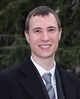
\includegraphics[height=1in]{images/vitae/lbenvenuti}}
\noindent {\bf Luca Benvenuti} is a PhD student and research assistant at Linz University where he studies particles characterization, both in the experimental and numerical way, 
applied to steel manufacturing processes. His academic and working experience on steel plants made him acknowledge the necessity to improve the design through numerical simulations 
optimization. Also his bachelor and master thes\={e}s have focused on both experimental and numerical work.
After his master thesis, he has done a three months' internship in an
international construction company to work as site engineer in the expansion project of the LISCO steel plant in 
the outskirt of Misrata. This experience gave him many skills, especially in field metallurgy engineering.

\vspace{2cm}

\parpic{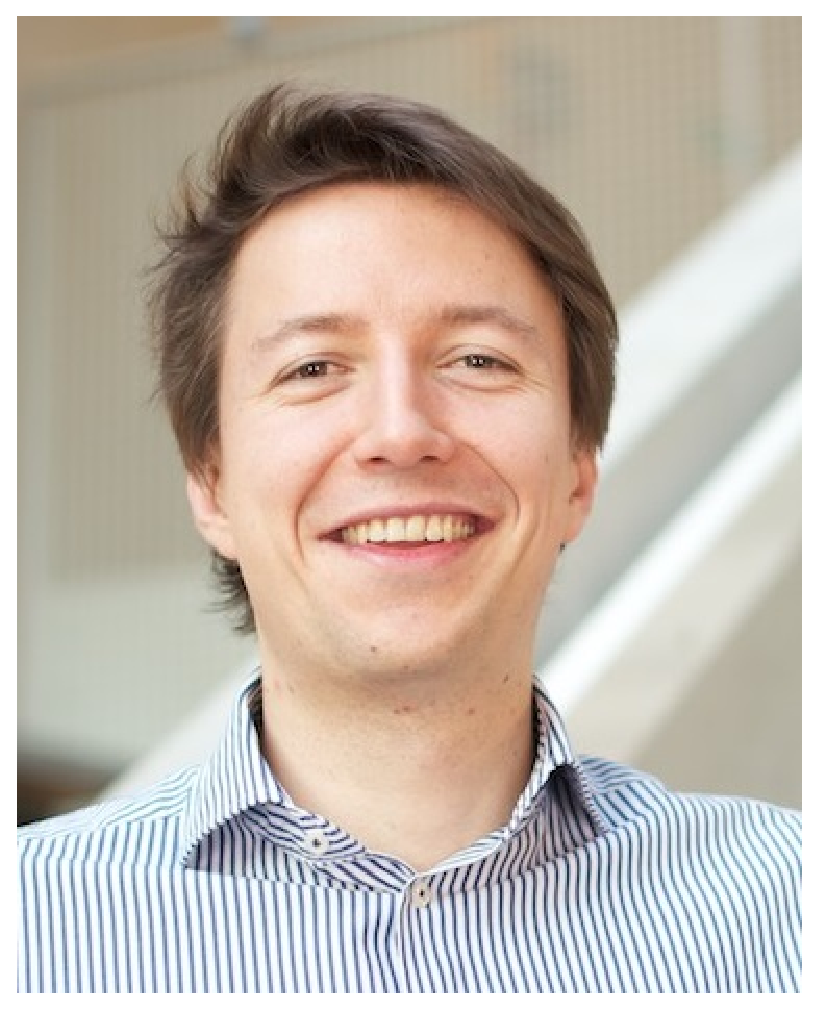
\includegraphics[height=1in]{images/vitae/ckloss}}
\noindent {\bf Christoph Kloss} received his Diploma in Mechatronics in 2007 and his PhD in Computational Fluid Dynamics in 2011, 
both at the Johannes Kepler University in Linz. From 2011 to 2014, he has been Senior Research Associate at the Department of 
Particulate Flow Modelling at the Johannes Kepler University (JKU), where he headed a DEM and CFD-DEM modelling team together 
with Dr. Goniva. Dr. Kloss is co-founder and core developer of the ``CFDEM\textregistered project'', where he is heading the development of the open source DEM code LIGGGHTS\textregistered
Dr. Kloss and Dr. Goniva founded DCS Computing in January 2012. DCS is now a leading company in providing simulation software, 
products and services in the field of DEM and CFD-DEM simulations for a variety of industries. Dr. Kloss is currently holding the position as director of DCS Computing.

\vspace{2cm}

\parpic{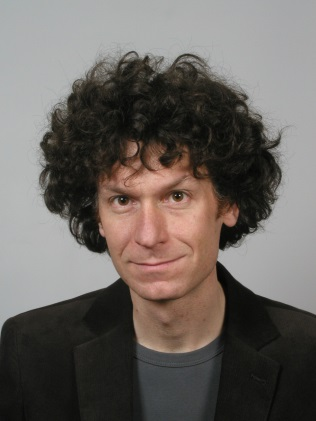
\includegraphics[height=1in]{images/vitae/spirker}}
\noindent {\bf Stefan Pirker} received his PhD in Computational Fluid Dynamics in 2001 at the Johannes Kepler University in Linz/Austria. 
In 2009 he was awarded a Christian-Doppler Laboratory on Particulate Flow Modelling, focusing on numerical modelling of particle laden flows. 
This involves development, experimental validation, application and finally open source distribution of hybrid particle laden flow models. 
After his habilitation in 2011, Stefan Pirker is currently heading the Department of Particulate Flow Modelling at the Johannes Kepler University in Linz/Austria.


\renewcommand\thefigure{\arabic{figure}}

\end{document}
